% Alternative Options:
%	Paper Size: a4paper / a5paper / b5paper / letterpaper / legalpaper / executivepaper
% Duplex: oneside / twoside
% Base Font Size: 10pt / 11pt / 12pt
\documentclass[a4paper, twoside, 11pt]{report}


% This file contains all the packages used in the template
% Remove or add new packages to suit your needs




%% Language %%%%%%%%%%%%%%%%%%%%%%%%%%%%%%%%%%%%%%%%%%%%%%%%%

% Bytt til norsk for å få norsk innholdsfortegnelse
\usepackage[USenglish]{babel} % norsk, francais, polish, spanish, ...

\usepackage[utf8]{inputenc}
\usepackage[T1]{fontenc}

%% Andre pakker %%%%%%%%%%%%%%%%%%%%%%%%%%%%%%%%%%%%%%%%%%%%%%%%%
\usepackage{hyperref}
\usepackage[sorting=none]{biblatex}
\usepackage{csquotes}
\usepackage{graphicx} %%For loading graphic files
\usepackage{amsmath}
\usepackage{amsthm}
\usepackage{amsfonts}
\usepackage{eso-pic}
\usepackage{transparent}

\usepackage{minted} % For including code
\usepackage{svg}
\usepackage{pdfpages}


%\usepackage{auto-pst-pdf} % Enables the psfrag tool
%\usepackage{psfrag}% Enables the psfrag tool
\usepackage{psfrag}
\usepackage{authblk}


%% For programming text input %%%%%%%%%%%%%%%%%%%%%%%%%%%%%%%%%%%%%%%%%%%%%%%%%

\usepackage[framed,numbered,autolinebreaks,useliterate]{mcode}
\usepackage{listingsutf8}
% Small fix for special characters
\lstset{literate=
  {á}{{\'a}}1 {é}{{\'e}}1 {í}{{\'i}}1 {ó}{{\'o}}1 {ú}{{\'u}}1
  {Á}{{\'A}}1 {É}{{\'E}}1 {Í}{{\'I}}1 {Ó}{{\'O}}1 {Ú}{{\'U}}1
  {à}{{\`a}}1 {è}{{\`e}}1 {ì}{{\`i}}1 {ò}{{\`o}}1 {ù}{{\`u}}1
  {À}{{\`A}}1 {È}{{\'E}}1 {Ì}{{\`I}}1 {Ò}{{\`O}}1 {Ù}{{\`U}}1
  {ä}{{\"a}}1 {ë}{{\"e}}1 {ï}{{\"i}}1 {ö}{{\"o}}1 {ü}{{\"u}}1
  {Ä}{{\"A}}1 {Ë}{{\"E}}1 {Ï}{{\"I}}1 {Ö}{{\"O}}1 {Ü}{{\"U}}1
  {â}{{\^a}}1 {ê}{{\^e}}1 {î}{{\^i}}1 {ô}{{\^o}}1 {û}{{\^u}}1
  {Â}{{\^A}}1 {Ê}{{\^E}}1 {Î}{{\^I}}1 {Ô}{{\^O}}1 {Û}{{\^U}}1
  {Ã}{{\~A}}1 {ã}{{\~a}}1 {Õ}{{\~O}}1 {õ}{{\~o}}1
  {œ}{{\oe}}1 {Œ}{{\OE}}1 {æ}{{\ae}}1 {Æ}{{\AE}}1 {ß}{{\ss}}1
  {ű}{{\H{u}}}1 {Ű}{{\H{U}}}1 {ő}{{\H{o}}}1 {Ő}{{\H{O}}}1
  {ç}{{\c c}}1 {Ç}{{\c C}}1 {ø}{{\o}}1 {å}{{\r a}}1 {Å}{{\r A}}1
  {€}{{\euro}}1 {£}{{\pounds}}1 {«}{{\guillemotleft}}1
  {»}{{\guillemotright}}1 {ñ}{{\~n}}1 {Ñ}{{\~N}}1 {¿}{{?`}}1
}


%% Line Spacing %%%%%%%%%%%%%%%%%%%%%%%%%%%%%%%%%%%%%%%%%%%%%
%\usepackage{setspace}
%\singlespacing        %% 1-spacing (default)
%\onehalfspacing       %% 1,5-spacing
%\doublespacing        %% 2-spacing


%% Other Packages %%%%%%%%%%%%%%%%%%%%%%%%%%%%%%%%%%%%%%%%%%%
%\usepackage{a4wide} %%Smaller margins = more text per page.
\usepackage{fancyhdr} %%Fancy headings
%\usepackage{longtable} %%For tables, that exceed one page

\usepackage{color}
\definecolor{darkgreen}{rgb}{0.3,0.6,0.3}

\parindent 0mm
\setlength{\oddsidemargin}{0mm}
\setlength{\evensidemargin}{0mm}
\setlength{\topmargin}{-20mm}
\setlength{\textwidth}{165mm}
\setlength{\textheight}{260mm}

\hypersetup{
   pdfauthor={UiA Mechatronics Student},
   pdftitle={Technical Report},
   pdfkeywords={report, mechatronics, University of Agder},
   pdfsubject={Project Report},
   colorlinks=true,
   citecolor=darkgreen,
   urlcolor=darkgreen,
   linkcolor=black,
   pdfstartview=Fit,
   pdfpagelayout=SinglePage,
   pdfcreator=pdflatex,
   pdfproducer=pdflatex
}
%\usepackage{wrapfig}

\newcommand{\subsubsubsection}[1]{\paragraph{#1}\mbox{}\\}
\setcounter{secnumdepth}{3}
\setcounter{tocdepth}{3}

%\newcommand{\subsubsubsection}[1]{\paragraph{#1}\mbox{}\\}
%\setcounter{secnumdepth}{4}
%\setcounter{tocdepth}{4}

\usepackage{tcolorbox}
\usepackage{algorithm, algorithmic} %

\usepackage{enumitem}% http://ctan.org/pkg/enumitem
%\Urlmuskip=0mu plus 1mu\relax

\usepackage{url}

%%% --- The following two lines are what needs to be added --- %%%
\setcounter{biburllcpenalty}{7000}
\setcounter{biburlucpenalty}{8000} % fixes urls

\addbibresource{bibliography.bib}

\begin{document}
%\rmfamily




\pagestyle{empty} %No headings for the first pages.


\begin{titlepage}


%%%% Select the correct front page by changing the reference below %%%% 

% Figures/Frontpage/forside_bachelor_eng.pdf
% Figures/Frontpage/forside_bachelor_nor.pdf
% Figures/Frontpage/forside_master_eng.pdf
% Figures/Frontpage/forside_master_nor.pdf

\AddToShipoutPicture*{
    \put(-4,0){
        \parbox[b][\paperheight]{\paperwidth}{%
            \vfill
            \centering
            % Change the reference in this line to change front page
            % forside_bachelor_eng.pdf, forside_bachelor_nor.pdf 
            % forside_master_eng.pdf, forside_master_nor.pdf
            
\includegraphics[width=1.275\textwidth]{Figures/Frontpage/forside_master_eng.pdf}%
            \vfill
        }
    }
    \put(0,0){%
        \transparent{0}\textcolor{white}{\rule{\paperwidth}{\paperheight}}
    }
}

%%%% Type in your data here %%%% 

\newcommand{\projectTitle}{This is the Title}
\newcommand{\projectSubTitlel}{ This thesis could have a subtitle that often could be somewhat longer than the title, and also stretch over several lines.}
\newcommand{\authors}{THE AUTHORS FULL NAME IN CAPITAL LETTERS}
\newcommand{\supervisor}{Supervisor's full name}

\newcommand{\projectYear}{2021}
\newcommand{\facultyName}{Faculty of Engineering and Science}
\newcommand{\departmentName}{Department of Engineering and Sciences}




%%%% Page Layout %%%% 
\begin{tabular}{p{12cm}}
                                            \\[5cm]
    \LARGE{\textsc{\textbf{\projectTitle}}} \\[1.5cm]
    \projectSubTitlel                       \\[2.5cm]
    \large{\authors}                        \\[9cm]
    \Large{SUPERVISOR}                      \\
    \supervisor
\end{tabular}



\vfill


\textbf{University of Agder, \projectYear} \\
\small{\facultyName \\
\departmentName}
\vspace{1cm}
\end{titlepage}

  
\clearpage

\pagenumbering{gobble}
\pagenumbering{roman}


\newpage



\large{\bf{Obligatorisk gruppeerklæring}} \\

{\small \hbadness=10000
Den enkelte student er selv ansvarlig for å sette seg inn i hva som er lovlige hjelpemidler, retningslinjer for bruk av disse og regler om kildebruk. Erklæringen skal bevisstgjøre studentene på deres ansvar og hvilke konsekvenser fusk kan medføre. Manglende erklæring fritar ikke studentene fra sitt ansvar.\\

\begin{center}
\begin{tabular}{ |p{1cm}|p{11.5cm}|p{1cm}|}
 \hline  
 
 1. & Vi erklærer herved at vår besvarelse er vårt eget arbeid, og at vi ikke har brukt andre kilder eller har mottatt annen hjelp enn det som er nevnt i besvarelsen. & Ja / Nei \\
 \hline
 2. & \textbf{Vi erklærer videre at denne besvarelsen:}
 \begin{itemize}
    \item Ikke har vært brukt til annen eksamen ved annen avdeling/universitet/høgskole innenlands eller utenlands.
    \item Ikke refererer til andres arbeid uten at det er oppgitt.
    \item Ikke refererer til eget tidligere arbeid uten at det er oppgitt.
    \item Har alle referansene oppgitt i litteraturlisten.
    \item Ikke er en kopi, duplikat eller avskrift av andres arbeid eller besvarelse.
 \end{itemize}& Ja / Nei \\
 \hline
 3. & Vi er kjent med at brudd på ovennevnte er å betrakte som fusk og kan medføre annullering av eksamen og utestengelse fra universiteter og høgskoler i Norge, jf. Universitets- og høgskoleloven §§4-7 og 4-8 og Forskrift om eksamen §§ 31.
 & Ja / Nei \\
 \hline
 4. & Vi er kjent med at alle innleverte oppgaver kan bli plagiatkontrollert.
 & Ja / Nei \\
 \hline
 5. & Vi er kjent med at Universitetet i Agder vil behandle alle saker hvor det forligger mistanke om fusk etter høgskolens retningslinjer for behandling av saker om fusk.
 & Ja / Nei \\
 \hline
 6. & Vi har satt oss inn i regler og retningslinjer i bruk av kilder og referanser på biblioteket sine nettsider.
 & Ja / Nei \\
 \hline
 7. & Vi har i flertall blitt enige om at innsatsen innad i gruppen er merkbart forskjellig og ønsker dermed å vurderes individuelt.
Ordinært vurderes alle deltakere i prosjektet samlet.
 & Ja / Nei \\
 \hline
\end{tabular}
\end{center}}

\bigskip

\large{\bf{Publiseringsavtale}} \\

{\small \hbadness=10000 Fullmakt til elektronisk publisering av oppgaven
Forfatter(ne) har opphavsrett til oppgaven. Det betyr blant annet enerett til å gjøre verket tilgjengelig for allmennheten (Åndsverkloven. §2).
\\
Oppgaver som er unntatt offentlighet eller taushetsbelagt/konfidensiell vil ikke bli publisert.\\

\begin{center}
\begin{tabular}{ |p{13cm}|p{1cm}|}
\hline
Vi gir herved Universitetet i Agder en vederlagsfri rett til å gjøre oppgaven tilgjengelig for elektronisk publisering: & Ja / Nei \\
\hline
Er oppgaven båndlagt (konfidensiell)? & Ja / Nei \\
\hline
Er oppgaven unntatt offentlighet? & Ja / Nei \\
\hline
\end{tabular}
\end{center}
}


\chapter*{Acknowledgements}
This template is meant as an example of how a technical report can be structured. Discuss
the table of content and the names of the chapters with the group members and supervisor
to suit your specific report.


\addcontentsline{toc}{chapter}{Acknowledgements}

\clearpage
\chapter*{Abstract}
\addcontentsline{toc}{chapter}{Abstract}

\clearpage

\tableofcontents
\cleardoublepage %The first chapter should start on an odd page.
\pagestyle{plain} %Now display headings: headings / fancy / ...

%List of Figures
\listoffigures
\addcontentsline{toc}{chapter}{List of Figures}
\clearpage
\textcolor{white}{.}
\thispagestyle{empty}
\newpage

%List of Tables
\listoftables
\addcontentsline{toc}{chapter}{List of Tables}
\clearpage

\textcolor{white}{.}
\thispagestyle{empty}
\newpage

\clearpage
\pagenumbering{arabic}





%\chapter{Introduction}
Autonomous vehicles have been used to complete hazardous tasks for several decades, like explosive disposal and work in radioactive areas. They are also used in automated manufacturing \cite{book}. Ensuring that the navigation of Autonomous ground vehicles (AGV) occurs safely is important to achieve efficient operation and avoid casualties. This applies equally to indoor navigation where collisions and obstacles represents significant risks. 

Normally, the UGVs use sensors of different modality - lidar for 3D perception of the surroundings and distance estimation, monocular camera for 2D perception backed by navigational and machine learning (ML) algorithms for autonomous navigation. However, the lidar used in this thesis possesses a fairly poor blind-zone, which results in objects that are too close and/or too close to the ground not getting detected. The consequence of this blind-zone could lead to costly and tragic accidents. This thesis aims reduce the blind-zone with the help of two radar modules, thus improving the safety of the systems navigation. The range data produced by the lidar are fused together with the range data from the radar modules to give the increased ability to detect close, low to the ground objects towards safer and collision free navigation.

In this thesis, Husky A200 \cite{husky-ugv} acts as an UGV, equipped with a 3D Ouster lidar \cite{ousterOS1datasheet}. Autonomous navigation is implemented trough the NAV2 package of the ROS2 framework \cite{doi:10.1126/scirobotics.abm6074}. Further, exploiting near field of view of TI radar module AWR1843BOOST \cite{awr1843boostintro} is fused with lidar to compensate for the near field blind zone of the lidar. The radars dependent on ROS1, therefore are all of the range sensors being run in ROS1. Finally, the ROS1 bridge is implemented to integrate the ROS1 part of the system with the ROS2 part making the communication among different sensors, and modules possible with the objective of attaining safer autonomous navigation with collision avoidance.

Work done in other project within lidar-radar fusion is presented in chapter \ref{chap:StateOfTheArt}. The chapter presents how the fusion of radar and lidar is used to enhance the different systems ability to detect and avoid objects. A camera based alternative to object detection is presented, but such systems require heavy processing power, and are susceptible to change in light. Lidars capability of precise range estimation combined with radars ability to detect objects can be used to increase the safety of autonomous navigation.

Chapter \ref{chap:Method} presents the methodology employed to address the challenge to overcome. The blind-zone issue is presented trough figures to give a visual understanding of the problem. The experimental setup is presented, first by giving an overview of the system and mentioning some less project specific components, then the range sensors, the Husky and the mounting system developed in this project is presented in more detail. The method chapter continues by providing a simplified representation of the system initialisation on the Husky's onboard computer. The ROS part of the system is discussed next, the ROS1 and the ROS2 part, and how they communicate with each other. 

The effect of the merging of radar and lidar ranging data is presented in chapter \ref{chap:TestingAndResults}, trough the presentation of testing and results. A navigation test have been done with only lidar and with both lidar and radar to compare the results. The results clearly depicts the advantages that the radars bring to the system. 

The discussions chapter, chapter \ref{chap:Discussions}, goes trough some challenges and decisions that were made during the project. The skid steering of the Husky UGV, and the problems it represents to the localisation is elaborated on. why two radar modules was used, and why they are positioned as they are are also discussed. It is also mentioned what effect mounting the radar modules differently may have. The mounting system for the radar modules went trough a failed prototype. The prototype mainly failed due to some dimensions being wrong. on the subject of radars, it is brought up why determining the field of view of the radar modules can be challenging.

Lastly, the thesis' conclusion is presented in chapter \ref{chap:Conclusions}. The chapter summarises the most important achievements and discoveries of this thesis. The increased safety of navigation trough lidar-radar fusion is the most important discovery, and ultematly the goal of the thesis.

\chapter{State of the art} \label{chap:StateOfTheArt}
Collision avoidance trough object detection is important for several types of systems, but especially important for autonomous systems, like self driving vehicles. Object detection has been made more accurate and reliable trough lidar-radar fusion. This chapter will go trough papers that discusses lidar-radar fusion for object detection and collision avoidance applications. 

The limitations of camera based object detection, like sensitivity to light intensity and heavy image processing, are explored in the first paper \cite{7579940}. A fusion scheme of lidar and radar are proposed as a solution to to the camera based system's shortcomings. Enhanced detection accuracy are achieved by exploiting by combining radar's ability to detect objects with the precise ranging data provided by lidar. This solution is especially suited for pedestrian detection and partially occluded scenarios.

The second paper \cite{8561087} discusses a method for lidar and radar fusion for the detection of occluded pedestrians. The paper presents occluded depth generation-based method that deals with pedestrian detection, occluded depth estimation and object detection. Object detection in occluded regions are done with radar.

Object detection and collision avoidance for autonomous driving are the focus of the third paper \cite{9951730}. False positives and missed detection are common errors in traditional object detection methods based on learning. The fusion of lidar and radar are utilised in two algorithms, presented in the paper, that addresses this issue. The first algorithm is based on occupancy grid detection, and the second utilises extended object tracking. The improved object detection achieved trough lidar-radar fusion is used by both methods, bettering collision avoidance.

obstacle detection and collision avoidance in a rural, unstructured environment, is achieved with a multi-sensor perception system in the fourth paper \cite{6916120}. Long range moving vehicle tracing is handled by radar, while a 3D lidar handles object detection and short range vehicle detection. Accurate detection and tracking of obstacles are used for effective collision avoidance.

The potential of lidar-radar fusion for object detection and collision avoidance are presented by all of the papers. The fusion of lidar and radar allows their strengths, like accurate ranging and object detection, to be combined improve accuracy and reliability of object detection and collision avoidance systems in autonomous driving.


%\chapter{Theory}
\section{Ranging sensors}
both lidar and radar are used in this project, 
\subsection{Time of flight}
The wave propagation speed for a wave is used in Time of flight sensors (TOF). Typical use case are electromagnetic - or acoustic waves. Equation \ref{eq:TOF1} is used to calculate the distance $d$ traversed by a wave \cite{introductionToMobileRobots}.   
\begin{equation} \label{eq:TOF1}
    d = c \cdot T
\end{equation}
where 
\begin{align*} 
d   & - distance \hspace{2mm} (usually \hspace{2mm} round-trip).\\
c   & - Propagation \hspace{2mm} speed \hspace{2mm} of \hspace{2mm} wave. \\
T   & - Time \hspace{2mm} of \hspace{2mm} fligth. \\
\end{align*}  
Time of flight sensors are often used to calculate the distance to a object by emitting a wave that are to be reflected of an object, back to the senor. Applying equation \ref{eq:TOF1} to the just described system would render double the distance to the object, because the wave will spend time travelling to the object and then back again. The distance are therefore calculated with equation \ref{eq:TOF2} \cite{introductionToMobileRobots}.
\begin{equation} \label{eq:TOF2}
    d = \frac{1}{2}c \cdot T
\end{equation}
This method of ranging is suitable for acoustic waves as they travel relatively slowly, compared with electromagnetic waves which travel about a million times faster. The electronics required for electromagnetic TOF-sensors are more expensive than the electronics required for acoustic TOF-sensors. Other ranging methods are therefore usually used instead of TOF when it comes to electromagnetic waves \cite{introductionToMobileRobots}.

\subsection{Continuous Wave}
A continuous wave can be emitted instead of burst of waves. The wave could be a simple sinusoidal wave that are emitted continuously. The received signal are mixed together with the emitted signal. Mixing of signals is done by multiplying them. Equation \ref{eq:x1x2} shows properties of a sent signal $x_1(t)$ and received signal $x_2(2)$.
\begin{equation} \label{eq:x1x2}
    x_1(t) = \sin(\omega_{1}(t + \phi_{1})), \hspace{1mm} x_2(t) = \sin(\omega_{2}(t + \phi_{2}))
\end{equation}
Then the following property is used:
\begin{equation} \label{eq:sin*sin}
    \sin(a) \cdot \sin(b) = \frac{1}{2}[\cos(a - b) - \cos(a + b)]
\end{equation}
Then $a$ is substituted with $\omega_{1}(t + \phi_{1})$, and $b$ with $\omega_{2}(t + \phi_{2})$:
\begin{equation} \label{eq:sin*sin}
    \frac{1}{2}[\cos(a - b) - \cos(a + b)] = \frac{1}{2}[\cos(\omega_{1}(t + \phi_{1}) - \omega_{2}(t + \phi_{2})) - \cos(\omega_{1}(t + \phi_{1}) + \omega_{2}(t + \phi_{2}))]
\end{equation}
The following expression described the mixed signal of $x_1$ and $x_2$:
\begin{equation} \label{eq:mix}
    x_1(t) \cdot x_2(t) = \frac{1}{2}[\cos((\omega_{1} - \omega_{2})(t + \phi_{1}-\phi_{2})) - \cos((\omega_{1} + \omega_{2})(t + \phi_{1} + \phi_{2}))]
\end{equation}

Figure \ref{fig:mix} illustrates how $x_1(t)$ and $x_2(t)$ might look like, and how their mixed signal looks like. The plot together with equation \ref{eq:mix} makes it obvious that the mixed signal consists of two frequency components, one greater than the other. The difference between the frequency components is usually much greater than that what is illustrated in figure \ref{fig:mix}, to a degree where they are easily separated by a low-pass filter. The third plot in figure \ref{fig:mix} displays both the mixed signal and the low-pass filtered mixed signal $LP(x_1(t) \cdot x_2(t))$. The low-pass filtered signal are described in equation \ref{eq:LP(mix)}.   

\begin{figure}[H]
\centering
\includesvg[scale=0.8]{Figures/matlab/mix.svg}
  \caption{Example of mixing of two signals}
  \label{fig:mix}
\end{figure}
\begin{equation} \label{eq:LP(mix)}
    LP(x_1(t) \cdot x_2(t)) = \frac{1}{2} 
 \cos((\omega_{1} - \omega_{2})(t + \phi_{1}-\phi_{2}))
\end{equation}

The frequency of the low-pass filtered signal is called the beat frequency, and it represents the Doppler shift \cite{douglas2022fmcw}. Doppler shift is produced when there is relative motion between sender/receiver and the detected object. However, only the motion along a axis that passes trough both sender/receiver and the detected object are measured \cite{cwradar}. This means that, in short, that Doppler shift is best detected when (for example) the detected object is either moving directly towards or away from the sender/receiver. Equation \ref{eq:nasa} describes how the Doppler shifted frequency relates to the relative velocity \cite{doppler_effect_nasa}.

\begin{equation} \label{eq:nasa}
    \omega_d = \omega_0 \frac{c}{c - v} 
\end{equation}
where 
\begin{align*} 
\omega_d   & - frequency \hspace{2mm} of \hspace{2mm} Doppler-shifted \hspace{2mm} signal.\\
\omega_0   & - frequency \hspace{2mm} of \hspace{2mm} emitted \hspace{2mm} signal.\\
c   & - Speed \hspace{2mm} of \hspace{2mm} wave \hspace{2mm} in \hspace{2mm} the \hspace{2mm} enviroment/medium.\\
v   & - Relative \hspace{2mm} velocity \hspace{2mm} between \hspace{2mm} sender/revciver \hspace{2mm} and \hspace{2mm} detected \hspace{2mm} object.\\
\end{align*}  
Equation \ref{eq:nasa} is rewritten to produce equation \ref{eq:doppler}.
\begin{equation} \label{eq:doppler}
    v = \left( 1 - \frac{\omega_0}{\omega_d} \right) c
\end{equation}

The beat frequency is the difference between the emitted and revived frequency. However, The difference is found inside a cosine function, which is symmetric meaning it has the peppery described by equation \ref{eq:cos}.

\begin{equation} \label{eq:doppler}
    \cos(-x) = \cos(x)
\end{equation}
Thus the beat frequency will be the same for a object moving towards the sender/receiver as for object moving at the same velocity but away form the sender/receiver. Thus the system cannot tell whether the object is moving closer or further form the sender/receiver, relative to the sender/receiver. The issue with not being able to determine direction can be solved by adding a signal orthogonal to the original signal emitted signal. The new part of the emitted signal is $90 \deg$ out of phase compared with the original signal. The new, out of phase and orthogonal, signal is the imaginary part of the now complex emitted signal. The relative direction of movement of the object can now be determined by observing whether the real part or the imaginary part of the now complex beat frequency is leading \cite{douglas2022fmcw}.

Distance between the sender/receiver and the object is found by considering the time shift between the emitted and revived signal. This system is only suitable for resolving distances shorter or equal one wavelength, due to the periodic nature of the emitted wave \cite{douglas2022fmcw}. This renders the system useless for measuring any significant distances, especially when using millimetre waves.   

\section{ROS}
Robot Operating System (ROS) is a open-source collection of software that are used as a framework for robotics. ROS has been in development in over ten years and it is an important part of the field of robotics. ROS is used in research, teaching and industrial applications. ROS contains many pre-made packages that can make it simpler to achieve advanced advanced functionality, like autonomous navigation \cite{WhyROS}. 

ROS is a software development kit (SDK) and not a operating system. ROS provides a standardised message-passing system that allows common hardware to be utilized by different software, like localisation algorithms. ROS comes equipped with tools to help with visualisation and launching software \cite{ROSEcosystem}. It is possible to configure autonomous robots with openly available software, without having to develop any complex algorithms.

ROS can be deployed on macOS, Windows, RTOS (Real Time Operating Systems) and Linux \cite{WhyROS}. The development of ROS are ongoing, and different distributions of ROS are released to ensure that the development does not break applications \cite{REP2000}. New ROS distributions are typically realised every year at world turtle day, may 23. distros, short for distributions, with long-term support are only realesed every second year, one month after a LTS distro of Ubuntu are released. 

\begin{figure}[H]
\centering
\includesvg[scale=1]{Figures/ros/ros-noetic-ninjemys.svg}
  \caption{Poster for the latest ROS distribution Noetic Ninjemys \cite{ROSLogo}}
  \label{fig:noeticLogo}
\end{figure}

The ROS distros seems to be somewhat similar and compatible, except for the ROS2 distros. ROS2 is a newer version of ROS with many improvements to its structure. ROS2 uses newer versions of C++ and Python, and differs in the tools utilised for creating and building packages \cite{ROSChanges}. ROS2 seems to be recommended over ROS (or ROS1) because it is newer. However, it also does not seem be as well tested as ROS1.

There are several aspects to ROS communication, but the most important ones to understand in this project are nodes, messages and topics. A node is essentially a program that can interact with the ROS-network. Different nodes may preform different tasks, for example, one node might be responsible for interfacing with the wheel actuators of a robot, while another one could be responsible for planning a path for the robot to take. Messages are the data which is communicated between nodes. Messages often follow a standardised structure such that different hardware and software can work together more easily. There is a standardised message type for 2D-Lidars called Laserscan, this can be utilised by ranging sensors and SLAM-like algorithms.  Topics are essentially the "channels" on which messages are sent. Topics are differentiated with arbitrary names, however it is common practice to name a topic something describing or something similar to the name of its message type. Nodes that sends out messages are publishing to topics, nodes that reads messages are subscribing to a topic. 

The simplest way to initialise a ROS-node is to first start the roscore, then run the "rosrun" command in the Ubuntu terminal. Running a ROS-node can look something like the following example.  
\mint{css}{rosrun "package" "node-name" "argument-name":="value"}
However, This method becomes cumbersome once there is a need for running several nodes, with their own arguments. Each node would require their own terminal window, in addition to the roscore. The solution to this issue is launch files. Launch files makes it possible 

\subsection{transforms tf2 or whatever}
\subsection{some nodes used?}
\chapter{Method}
\section{Problem}

\section{Tools}
This section will explain the tools used in this project, like ROS, ubuntu, the lidar radars husky....

\section{Hardware}

\begin{figure}[H]
    \centering
    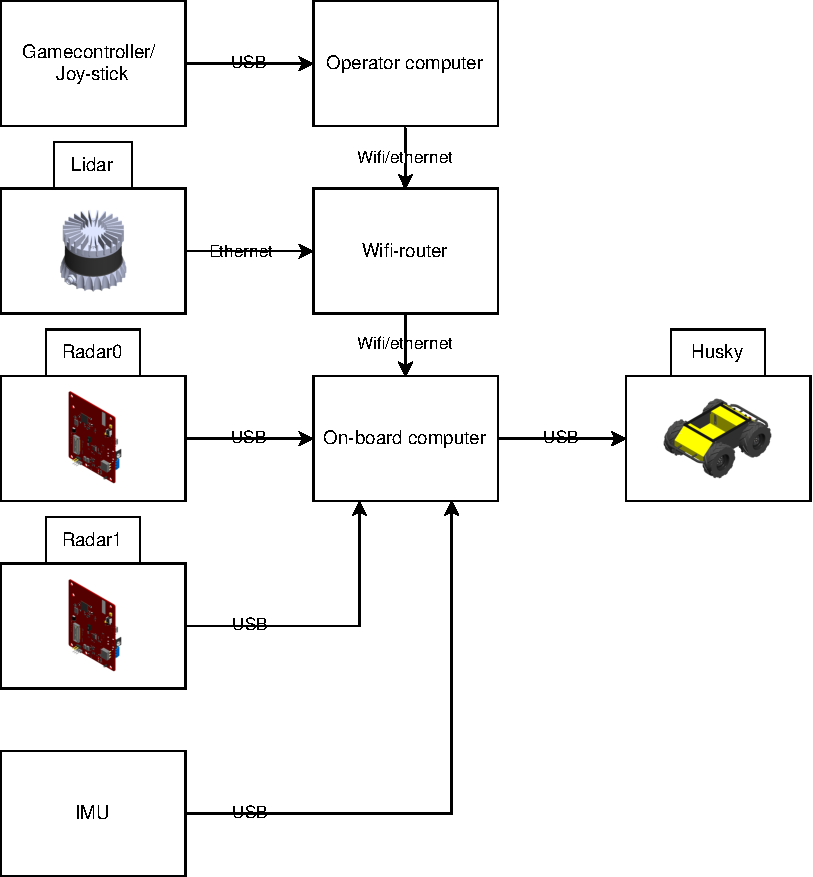
\includegraphics[scale=1]{Figures/draw.io/hardwareBlockDiagram.drawio.pdf}
    \caption{Hardware diagram of system}
    \label{fig:HWdiagram}
\end{figure}

\begin{figure}[H]
    \centering
    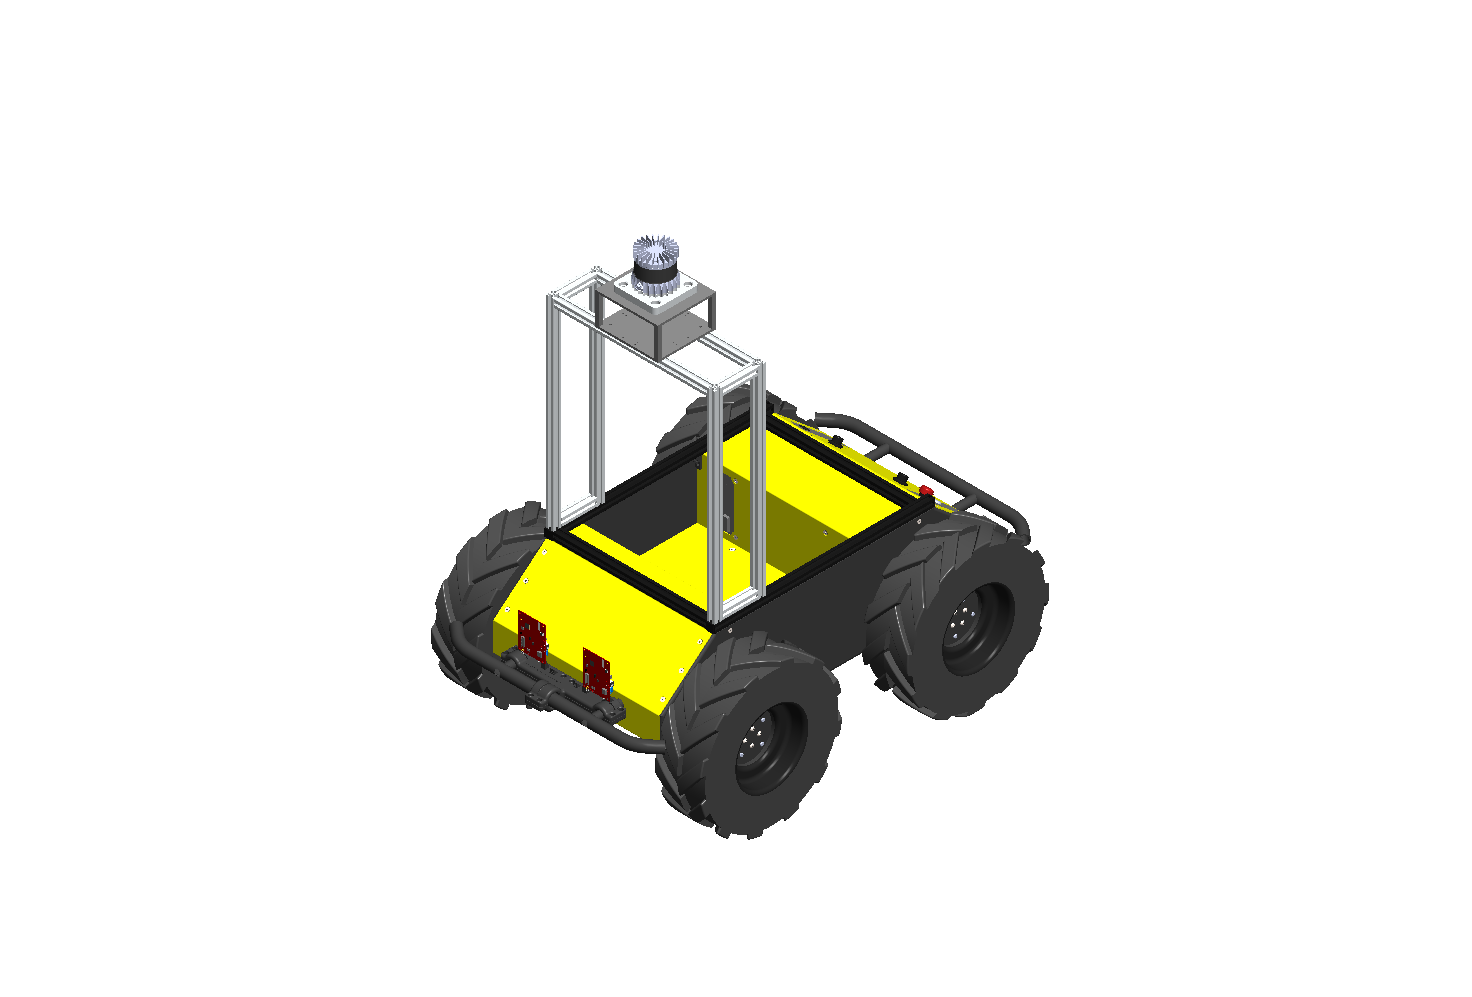
\includegraphics[scale=0.5]{Figures/CAD/huskyWithSensors.PNG}
    \caption{Hardware diagram of system}
    \label{fig:HWdiagram}
\end{figure}
\subsection{Sensors}
\subsubsection{Lidar}

\subsection{Sensors}
\subsubsection{Lidar}

\subsubsection{Radar}
\subsubsubsection{Mount}
\subsubsection{IMU}
\subsection{Husky A200}
\subsection{Logitech F710}
\subsubsection{Kinematics}
\subsection{Computers}

\section{ROS system}
The work done in this project is a continuation and expansion of previous work \ref{Appdix:MAS513}. This previous work consisted of, among other things, configuring a Unmanned Ground Vehicle (UGV) along with sensors, in ROS2. There was therefore a desire to continue the work in this project in ROS2. The issue was that the pre-made package for the radar-modules was made for ROS1. The migration methods described on the official ROS2 documentation where attempted (described in \cite{ROSMigrationGuide}). Attempts where also made on using Amazon's tools for migrating ROS1 to ROS2 (described in \cite{ROSMigrationGuide}). Attempts on migrating the radar-package to ROS2 was ultimately abandoned. The perception system was implemented i ROS1, then the ROS1 bridge was utilised for communicating with the rest of the system which runs on ROS2.

\subsection{ROS1 system}
The ROS1 system is responsible for reading in data from a 3D-Lidar \ref and two radar-modules \ref, combining data and sending it on a format can be used for navigation purposes. The navigation system used in this project, and in \ref{Appdix:MAS513}, relays on the Laserscan message sent on the "/scan"-topic. The ROS1 system must provide the ROS2 system with the proper messages on the "/scan"-topic. Figure \ref{fig:rqt:ros1_noBridge} displays a rqt node-graph of the ROS1 system. The system is divided in to four main parts, which will be explained in the following parts.

Figure \ref{fig:simpleRos1Rqt} simplified presentation of the visualisation system running on ROS1. The nodes are represented by the red ovals, the green rectangles depicts the topics and the blue rectangles are used for groups, or common name spaces. All of the nodes, topics and "groups" that exists in a group share a common name space, like "$/namespace"$. For example, all the entities in the "$/radar0$" group begin their name with "$/radar0$". This naming convention serves two purposes, it allows , in a way, all the sensors to publish to the same topic name. For example, all of the sensors publishes to the "$/PointCloud$" topic, but no issues with similar names arises because they all use different naming prefixes. The second purpose is to allow the system to be viewed in a intuitive and structured way in the rqt node-graph.  

\begin{figure}[H]
\centering
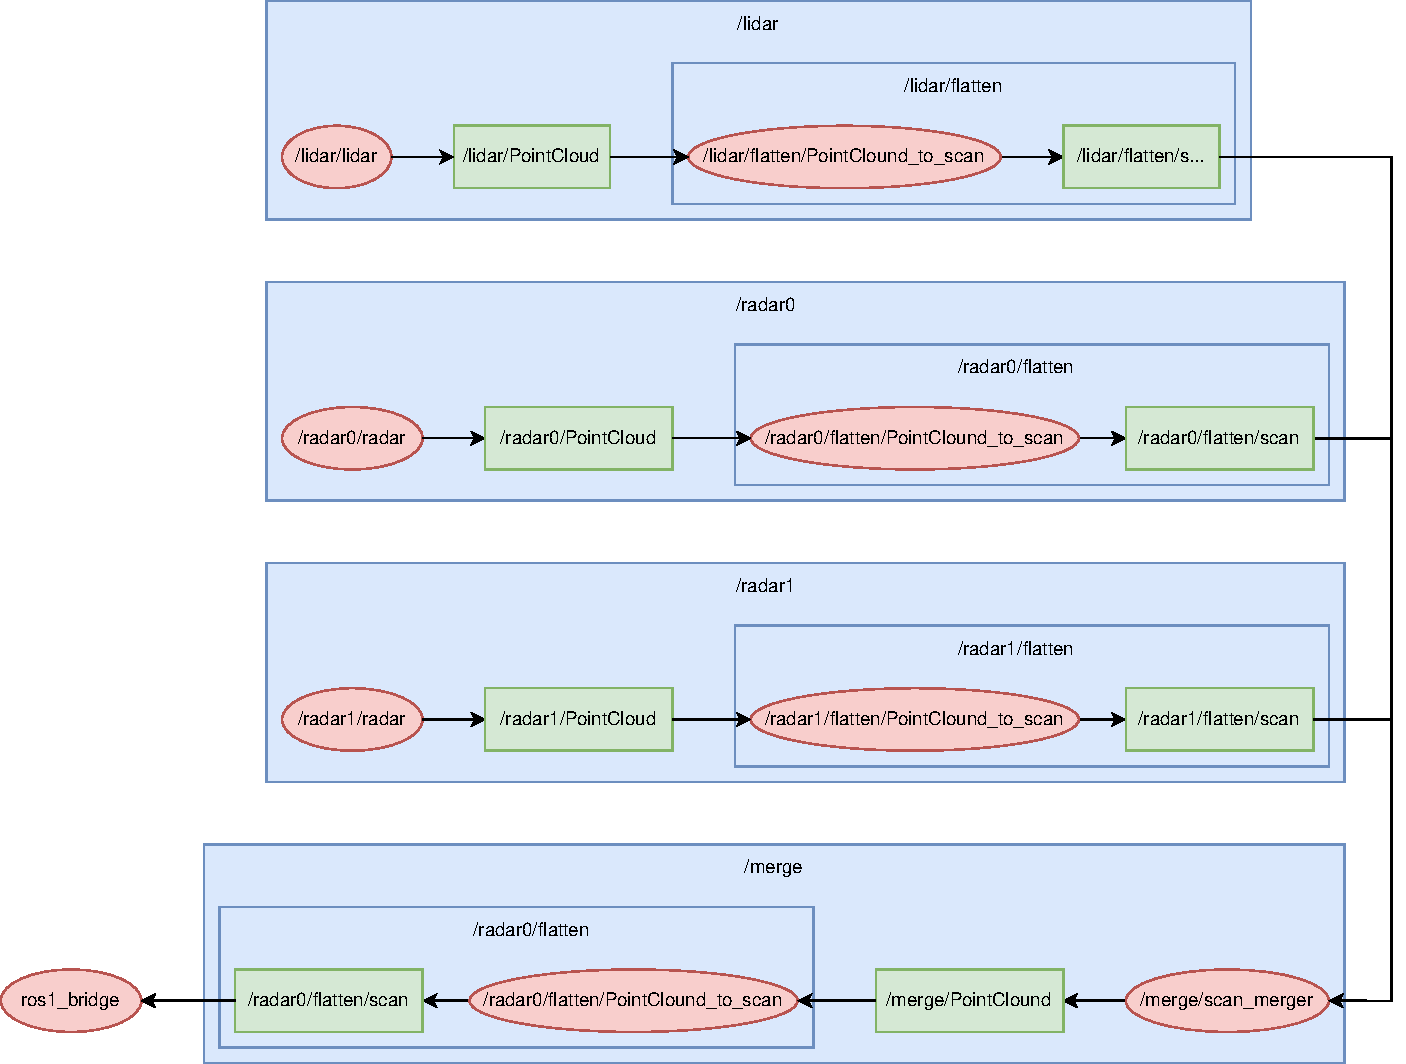
\includegraphics[scale=0.65]{Figures/draw.io/sipleRqtRos1.drawio.pdf}
  \caption{Simplifyed node-graph of ROS1 system}
  \label{fig:simpleRos1Rqt}
\end{figure}


\subsubsection{Packages}

\subsubsection{\textit{launch}}
The system is brought up with the help of launch files. One launch file (two in practice) is used to launch the entire ROS1 system, except the ROS1 bridge. The master launch file(s) are responsible for calling upon other "sublaunch" files. The sublaunch file system allows similar functionality to be re-used, similarly to how functions might be used in c or Python. All of the groups depicted in figure \ref{fig:simpleRos1Rqt} has a sublaunch file associated with it. \textit{viz.launch} is launched if the argument \textit{viz} is set to \textit{true} when 

The sublaunch files takes in arguments, which can be passed over to the elements being launched. The arguments can be passed to the sublaunch file when it is called, but there are default settings that are applied for the arguments not specified when the launch file is ran. The arguments are passed down either to the nodes or the launch files that are called upon. Some of the arguments are used so that one launch file can called by different launch files without them interfering with each other, by for example changing the prefix on nodes and topics, like mentioned above. The following sections will go over the different launch files.

\subsubsubsection{\textit{flatten.launch}}\label{subsubsec:flatten.launch}
"\textit{flatten.launch}" is used to launch the \textit{pointcloud\_to\_laserscan\_node} 
node of the \textit{pointcloud\_to\_laserscan} package. The \textit{pointcloud\_to\_laserscan\_node} node is used to convert a 3D point cloud to a 2D laser scan \cite{pcl_ros}. The conversion will include objects within a given height range set by two arguments, "\textit{min\_height}" and "\textit{max\_height}". The \textit{pointcloud\_to\_laserscan\_node} node subscribes to the \textit{cloud\_in} topic, and expect a message on the \textit{sensor\_msgs/PointCloud2} message format \cite{pcl_ros}. \textit{remap} is used to make the node more generic by allowing the subscribed topic to be set by an argument. The node publishes on the \textit{scan} topic with the \textit{sensor\_msgs/LaserScan} message format. The node is launched within a group with a name space (NS) which adds a NS prefix to the name of the launched node and the published topic.

\subsubsubsection{\textit{lidar.launch}}\label{subsubsec:lidar.launch}
\textit{lidar.launch} is responsible for launching and configuring the nodes for the Lidar. A launch file that are included in the packages for the Lidar is used to bring up the Lidar system, which  consists of several nodes. Some arguments are passed to the Lidar launch file, some notable are the \textit{ouster\_ns} - and the  \textit{timestamp\_mode} arguments. The \textit{ouster\_ns} argument is responsible for the second \textit{/lidar} group within the \textit{/lidar} group as seen in figure \ref{fig:Appdix:rqt:ros1_noBridge}. However, this \textit{/lidar/lidar} are represented by a single node in the simplified node graph in figure \ref{fig:simpleRos1Rqt}. TIME\_FROM\_ROS\_TIME A remapping of the standard point cloud topic name is done to make it configurable, trough an argument, and more fitting with the naming scheme of the rest of the system. \textit{flatten.launch} (\ref{subsubsec:flatten.launch}) is called upon, and the \textit{input\_PointCloud} argument is set to the same topic name as the point cloud form the Lidar are published on. \textit{min\_height} and \textit{max\_height} are set to $-1 m$ and $1 m$ respectively. These values does not consider the robot's structure, and would ideally be set such that the lower limit is close to the ground, and the upper limit a little above the Lidar. However, the values used seems to work fine. 

A \textit{static\_transform\_publisher} node form the \textit{tf2\_ros} package is used to crate a "dummy"-frame on top of the frame for the Lidar provided by the Lidar-package. This done so that the name of the frame can be altered trough an argument, making it more generic. A second \textit{static\_transform\_publisher} node is used to relate the Lidars position to the rest of the system. The \textit{parent\_link\_name} argument is used to set the name of the parent link of the Lidar, so it can be associated with any frame. The \textit{pos} argument describes the transform between the Lidar's frame and the parent frame. See \ref{Appdix:lidar.launch} to see the code for the launch file.

\subsubsubsection{\textit{radar.launch}}\label{subsubsec:radar.launch}
\textit{radar.launch} has a somewhat similar structure to \textit{lidar.launch} \ref{subsubsec:lidar.launch}, but is used for launching the radars and not the Lidar. \textit{radar.launch} is a heavily modified version of the launch file intended for the radar-modules, included with the radar package (\textit{awr1843boost\_test.launch}). The original launch file did not allow certain arguments to be altered, thus it was necessary to create a new launch file, instead of calling the original. A group with a configurable NS is set for the nodes and topics, similar to the other launch files. A remapping of the standard point cloud topic name is done for similar reasons as in \textit{lidar.launch} \ref{subsubsec:lidar.launch}, but also to allow multiple radar modules to be launched. The \textit{ti\_mmwave\_rospkg} node of the \textit{ti\_mmwave\_rospkg} package is responsible for interfacing with the radar modules, by publishing their data as point clouds on the ROS network. The \textit{command\_port} - and the \textit{data\_port} argument has been altered to \textit{/dev/ttyACM\$(arg command\_port\_number)} and \textit{/dev/ttyACM\$(arg data\_port\_number)}, respectively. These arguments is used to inform the node about the file path of the communication link to the radar module, thus it is critical that these can be changed when more than one radar module is used. The file path arguments are set such that only a integer needs to be passed in to the launch file, the rest of the file path does not change (at least for the systems utilised in this project). The \textit{frame\_id} argument is used to set the name of the frame of which the centre of the radar sits. \textit{frame\_id} is set to be \textit{\$(arg radar\_ns)/atenna\_center}, which is a frame located approximately at the centre of the antenna patch of the radar URDF, which will be explained further below. The rest of the arguments are similar to those in the original launch file. 

The \textit{mmWaveQuickConfig} node of the \textit{ti\_mmwave\_rospkg} package is used to provide the radar module with a configuration file. This seems to be a necessary step for the radar to start operating. Radar configuration files can be created with a web tool, but a pre-made configuration file is used, just as in the original launch file. Two \textit{static\_transform\_publisher} nodes are used for similar purposes as those used in \textit{lidar.launch} \ref{subsubsec:lidar.launch}. The points published by the \textit{ti\_mmwave\_rospkg} node are practically speaking two dimensional. However, the points are published at the \textit{sensor\_msgs/PointCloud2} message format. \textit{flatten.launch} \ref{subsubsec:flatten.launch} is used similarly as in \textit{lidar.launch} \ref{subsubsec:lidar.launch}. The \textit{robot\_state\_publisher} node of the \textit{robot\_state\_publisher} package is used make a description of the radar module available on the ROS network. This description is defined in a URDF file. Some remapping are done to allow multiple descriptions to be initialised at the same time. The parameter \textit{tf\_prefix} is set to avoid name conflicts between the frames of different descriptions. See \ref{Appdix:radar.launch} to see the code for the launch file.

\subsubsubsection{\textit{merge.launch}}\label{subsubsec:merge.launch}
The \textit{merge.launch} launch file is used to launch the \textit{laserscan\_multi\_merger} node of the \textit{ira\_laser\_tools} package. This node subscribes to a list of \textit{sensor\_msgs/LaserScan} type topics provided by the \textit{laserscan\_topics} argument, and combines them. The node publishes a point cloud and a laser scan, but the laser scan provided by the node did not behave as expected. However, the point cloud seems to consist of data similar to the input messages, thus this was used. The merged point cloud gets passed in to \textit{flatten.launch} \ref{subsubsec:flatten.launch}, which produces the final, merged, scan message.

\subsubsubsection{\textit{mount.launch}}\label{subsubsec:mount.launch}
The \textit{mount.launch} launch file is used to make a description of the radar mount available on the ROS network, is a similar manner as in \textit{radar.launch} \ref{subsubsec:radar.launch}. The URDF-file of the mount produces three frames that represent locations where radar modules can be mounted. \textit{static\_transform\_publisher} nodes are used to place frames on top of the existing, where the names of the new frames can be set with arguments. A \textit{static\_transform\_publisher} node is used to create a transform between the base of the mount description and the rest of the system.

\subsubsubsection{\textit{viz.launch}} 
\textit{viz.launch} is used to launch two visualisation tools of ROS, \textit{rqt} and {rviz2}. \textit{rqt} appears to open as it was closed, thus no "special" configuration is required. \textit{rviz} on the other hand will (seemingly) automatically open a standard configuration, which forces the user to configure \textit{rviz} each time it is opened. A file containing settings for \textit{rviz} has been created and this file are called when \textit{rviz} gets launched, this solves solves the issue with having to apply settings each time the program is opened.

\subsubsubsection{\textit{launchNoRadar1.launch}}\label{subsubsec:launchNoRadar1.launch}
\textit{launchNoRadar1.launch} is one of two launch files that are launched "manually" and not trough a different launch file. These can be viewed as "main" launch files, as they call other launch files, and does not initialise any nodes directly. \textit{viz.launch} is launched if the argument \textit{viz} is set to \textit{true} when \textit{launchNoRadar1.launch} is called. \textit{mount.launch} is launched before the radars to ensure that the mount frames exists when the radars are launched. The mount is rotated about the $x$ axis, of the base frame of the robot, with $\frac{2}{\pi} rad$ trough the \textit{pos} argument. \textit{radar.launch} \label{subsubsec:radar.launch} is called with the argument \textit{radar\_ns} set to \textit{radar0}. The \textit{parent\_link\_name} argument is set to \textit{radar\_pos1}, and the \textit{command\_port\_number} - and \textit{data\_port\_number} arguments are set to \textit{0} and \textit{1}, respectively. The \textit{lidar.launch} \ref{subsubsec:lidar.launch} launch file is called with the \textit{pos} argument set such that the Lidar are placed and rotated propperly. The $x$, $y$ and $z$ coordinates of the radar were obtained by summing the transforms and the URDF of the Lidar from the base project. The Lidar are mounted backwards, this is corrected by rotating it $\pi rad$ about the $z$ axis. Lastly, the \textit{merge.launch}\ref{subsubsec:merge.launch} launch file is called. The only argument that is passed passed to the \textit{merge.launch} \ref{subsubsec:merge.launch} launch file is the \textit{command\_port\_number} argument, this is configured so it share the base frame with the rest of the ROS1 system.

\subsubsubsection{\textit{launchRadar1.launch}}\label{subsubsec:launchRadar1.launch}
\textit{launchRadar1.launch} and \textit{launchNoRadar1.launch} \ref{subsubsec:launchNoRadar1.launch} where originally part of the same launch file, but they where split up due to some technical issues. The process of launching the radars seem to consist of two steps, configuration and reading data. The issue seems to surround the configuration part. The behaviour of the configuration appears to be unpredictable, and it can take several launching attempts and restarts of the radar modules to successfully launch the radars. The radars have been launched by at a point, but is was a lot less reliable than the current solution. The Github pages associated with the \textit{ti\_mmwave\_rospkg} package seems to suggest that is difficult to launch several radars at the same time due to conflicts with the USB-communication. The second radar is launched by calling \textit{radar.launch} \ref{subsubsec:radar.launch}, but this time with different arguments. The \textit{radar\_ns} argument is set to \textit{radar1}, the \textit{radar.launch} - and the argument is set to \textit{2} and \textit{3}, respectively. The \textit{radar.launch}

\subsection{ROS2 system}
The ROS2 system 

\subsubsection{\textit{uia\_husky\_0776}}
\textit{uia\_husky\_0776} is not a package, but a collection of packages that are used to operate the Husky. \textit{uia\_husky\_0776} exists as a Github repository and it is sheared between the three projects. This repository was created mostly by the Øvsthus-project, as this required (at some point) the Husky to be operated trough Galactic instead of Foxy, which was used in the base project. This repository is quite similar to, and based upon the repository used for the base project. 
%\subsubsection{\textit{husky\_group}}
The \textit{husky\_group} package that can be used to launch the Husky, both physically and in simulation, and several launch - and parameter files used in this project are modified version of launch - and parameter files from this package. The \textit{uia\_master\_husky} package is, in short, a modified version of Clearpath's ROS2 Galactic packages for the Huksy, where the modifications where made by Øvsthus. The \textit{um7} package is used to communicate with the IMU, and to make its data available on the ROS2 network. The \textit{serial} package is simply used by the \textit{um7} package for serial communication. The process of installing and running the contests of the \textit{uia\_husky\_0776} repository is explained quite well on its \href{https://github.com/orjano-max/uia_husky_0776}{Github page}.

\subsubsection{\textit{ros1\_bridge}}
The \textit{ros1\_bridge} package contains a network bridge that allows messages to be exchanged between ROS1 and ROS2 \cite{ros1_bridge}. The bridge will only carry messages in situations where one side sends a message that gets subscribed to on the other side, at least by default. This done to increase computational efficiency. The bridge can be tested by running the command below in ROS2 \cite{ros1_bridge}. 

\begin{tcolorbox}[width=\textwidth,colback={black},colupper=white, title={ubuntu terminal},colbacktitle=gray!125,coltitle=gray!50]\label{shell:echo}    
   \mint{shell}{ros2 topic echo <topic-name> <topic-type>}
\end{tcolorbox}  

Running this command will cause a topic to be subscribed to, and its messages to be displayed in the same terminal as the command was run in. \textit{<topic-name>} should be replaced with the name of the desired topic, and \textit{<topic-type>} with the name of the \href{https://docs.ros.org/en/noetic/api/sensor_msgs/html/msg/}{message type}. It is critical that the \textit{/scan} topic are "translated" by the bridge, thus this is what the described method was used for. The \textit{/scan} topic are associated with the \href{https://docs.ros.org/en/noetic/api/sensor_msgs/html/msg/LaserScan.html}{\textit{sensor\_msgs/LaserScan}} message format. Thus the following command is run:

\begin{tcolorbox}[width=\textwidth,colback={black},colupper=white, title={ubuntu terminal},colbacktitle=gray!125,coltitle=gray!50]\label{shell:echo1}    
   \mint{shell}{ros2 topic echo /scan sensor_msgs/LaserScan}
\end{tcolorbox} 

The \textit{/scan} topic should be visible in both \textit{rqt} and \textit{rviz2}, in ROS2, after running this command (assuming it is visible in ROS1). 

\subsubsubsection{Install and run}
The package can be installed differently depending on the use case. Installing the pre-built packages is convenient in this project, as the messages used are relayed properly with this instalment of the bridge. The \textit{ros1\_bridge} package can be installed by running the following command: 

\begin{tcolorbox}[width=\textwidth,colback={black},colupper=white, title={ubuntu terminal},colbacktitle=gray!125,coltitle=gray!50]\label{shell:echo1}    
   \mint{shell}{sudo apt install ros-<ros2 distro>-ros1-bridge}
\end{tcolorbox} 

Where \textit{<ros2 distro>} should be replaced with the name ROS2 distribution used, this would be \textit{Galactic} in this project. Installing the \textit{ros1\_bridge} for \textit{galactic} can be done by running the following command:

\begin{tcolorbox}[width=\textwidth,colback={black},colupper=white, title={ubuntu terminal},colbacktitle=gray!125,coltitle=gray!50]\label{shell:echo1}    
   \mint{shell}{sudo apt install ros-galactic-ros1-bridge}
\end{tcolorbox} 

The bridge, like other packages, have to be sourced before it can be run, but unlike most packages, the bridge requires both ROS1 and ROS2 to be sourced. The bridge itself is sourced together with ROS2, as the binary packages was installed. The following sequence of command can be used to run the bridge.

\begin{tcolorbox}[width=\textwidth,colback={black},colupper=white, title={ubuntu terminal},colbacktitle=gray!125,coltitle=gray!50]\label{shell:echo1}    
   \mint{shell}{source /opt/ros/noetic/setup.bash}
   \mint{shell}{source /opt/ros/galactic/setup.bash} 
   \mint{shell}{ros2 run ros1_bridge dynamic_bridge}
\end{tcolorbox} 

\subsubsection{\textit{teleop\_twist\_joy}}
The \textit{teleop\_twist\_joy} package allows the Husky to be remote controlled by a game-controller, or a joy-stick. This function was served by a different joy-stick package in the base project, but this solution stopped working after the SBC where re-flashed. The package comes with a launch file that launches two nodes, one reads the inputs form joy-stick an publishes this to the ROS2 network at the \textit{/joy} topic, the other subscribes to the \textit{/joy} topic and translates button presses to velocity messages.

\subsubsection{\textit{slam\_toolbox}}
\subsubsection{\textit{nav2\_bringup}}


%\begin{figure}[H]
%\centering
%\includesvg[scale=0.14]{Figures/ros/ros1graph_noBridge.svg}
%  \caption{rqt node-graph of ROS1 system (see %\ref{Appdix:rqtROS1NB} for a bigger figure)}
%  \label{fig:rqt:ros1_noBridge}
%\end{figure}



\begin{table}[h!]
\centering
\begin{tabular}{c |c| c}
                &   Laptop              &   SBC and Laptop  \\
    \hline
    Ubuntu      &   18.04 (Bionic)      &   20.04 (Focal)   \\
    \hline
    ROS1        &   Melodic Morenia     &   Noetic Ninjemys \\  
    \hline
    ROS2        &   Eloquent Elusor     &   Galactic Geochelone\\
\end{tabular}
\caption{Table to test captions and labels.}
\label{table:1}
\end{table}
%\chapter{Testing and results}\label{chap:TestingAndResults}
The main testing of the system was preformed in the machine hall of UiA. Figure \ref{fig:testSetup} illustrates the test setup. The Husky (left side of picture) are positioned in front of a backpack, placed outside of the FOV of the lidar, (right side of picture). The test was run with and without the radars active, to see the effect the radars give the system. The test procedure consisted of first mapping the area with SLAM, by driving the Husky around manually, then the test setup would be assumed. NAV2 would be asked to drive to a location behind the backpack to test whether the Husky would crash in to the backpack or not. 

\begin{figure}[H]
    \centering
    \includegraphics[width=1\textwidth]{Figures/testSetup.png}
    \caption{Test setup. Husky on left positioned towards backpack (right). The backpack is propped up by a battery (black and grey box).}
    \label{fig:testSetup}
\end{figure}

Figure \ref{fig:slamWithRadarRos2} displays the ROS2 part of the system trough a screenshot of Rviz2, this will be explained further below. Figure \ref{fig:slamWithRadarRos1} displays the ROS1 part of the system, in the form of a screenshot of Rviz. The radar mount can bee seen with two radar modules mounted to it, some distance away form the base link/base reference frame. Three colourful spheres can be viewed directly above the radar modules, these represent ranging data from the radars. More radar data/points can bee seen can be observed near the right edge of the figure (\ref{fig:slamWithRadarRos1}), at the upper half. The tree points just above the radar modules seem to be static and a product of some kind of noise or error, they are therefore "filtered" out by the \textit{flatten.launch} functionality (see \ref{subsubsec:flatten.launch}). The smaller, less colourful points (mostly orange, yellow and green) represents the 3D pointcloud of the lidar. Each square that makes up the grid seen in the figure measures $10 cm$ by $10 cm$. 

Figure \ref{fig:slamWithRadarRos2} displays the ROS2 part of the system, in the form of a screenshot of Rviz2. The husky can bee seen near the middle of the figure, sitting on top a light grey surface with black squares (mostly) separating the light grey area from a dark grey area. These grey and black areas represents the map produced by SLAM. Light grey represents unobstructed areas where the Husky can navigate, black are occupied areas and dark grey areas are unknown/unobserved areas. The difficult to spot, white points near the black areas represent the merged range data of the ROS1 system (two radar modules and a lidar). Figure \ref{fig:radarAndLidarPointsInRos2} better illustrates the merged range data. Each square that makes up the grid seen in the figure measures $1 m$ by $1 m$.

\begin{figure}[H]
    \centering
    \begin{minipage}[b]{0.49\textwidth}
        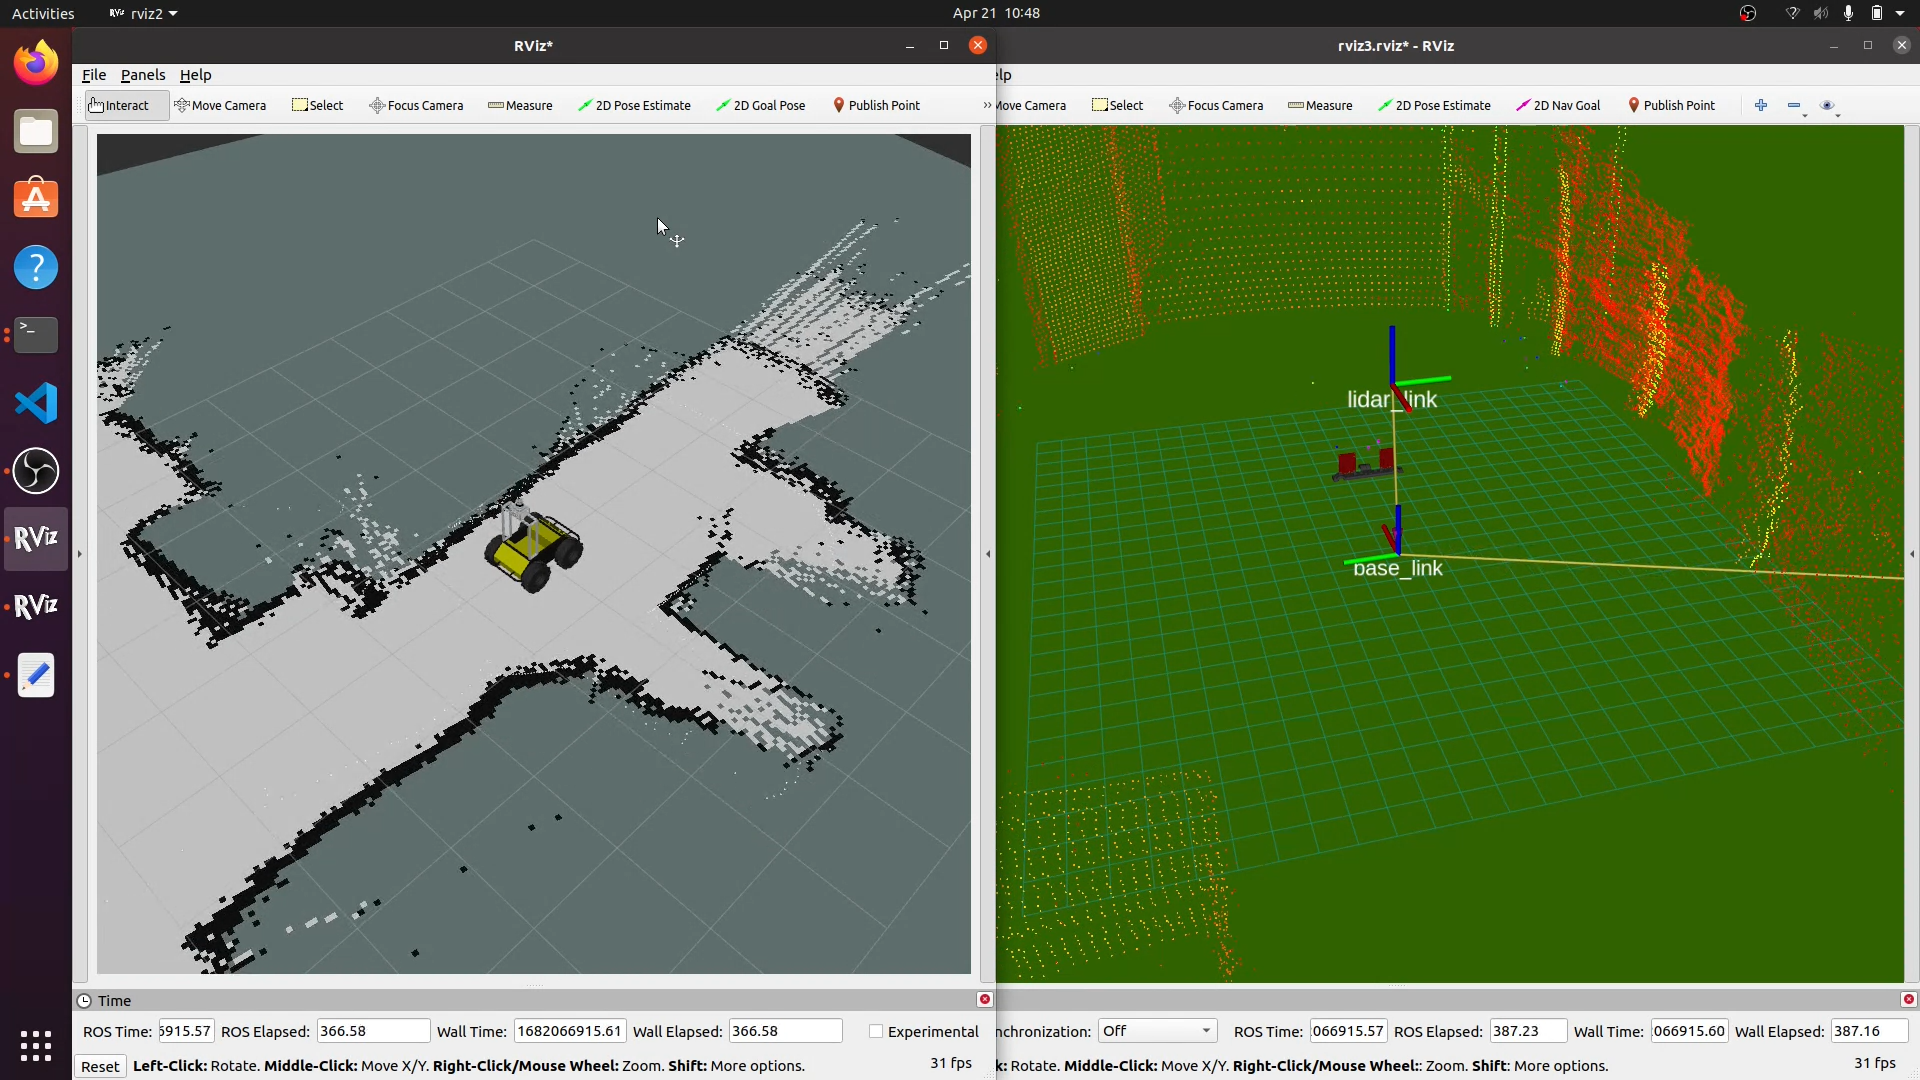
\includegraphics[width=\textwidth,trim={7cm 4cm 25cm 7cm},clip]{Figures/slamWithRadar.png}
        \caption{Zoomed in view of Rviz2 showing the Husky in a map produced by SLAM. Small dots around the black areas represent merged range data from ROS1 (seen in figure \ref{fig:slamWithRadarRos1}). Based on figure \ref{fig:slamWithRadar}.}
        \label{fig:slamWithRadarRos2}
    \end{minipage}
    %\hfill
    \begin{minipage}[b]{0.49\textwidth}
        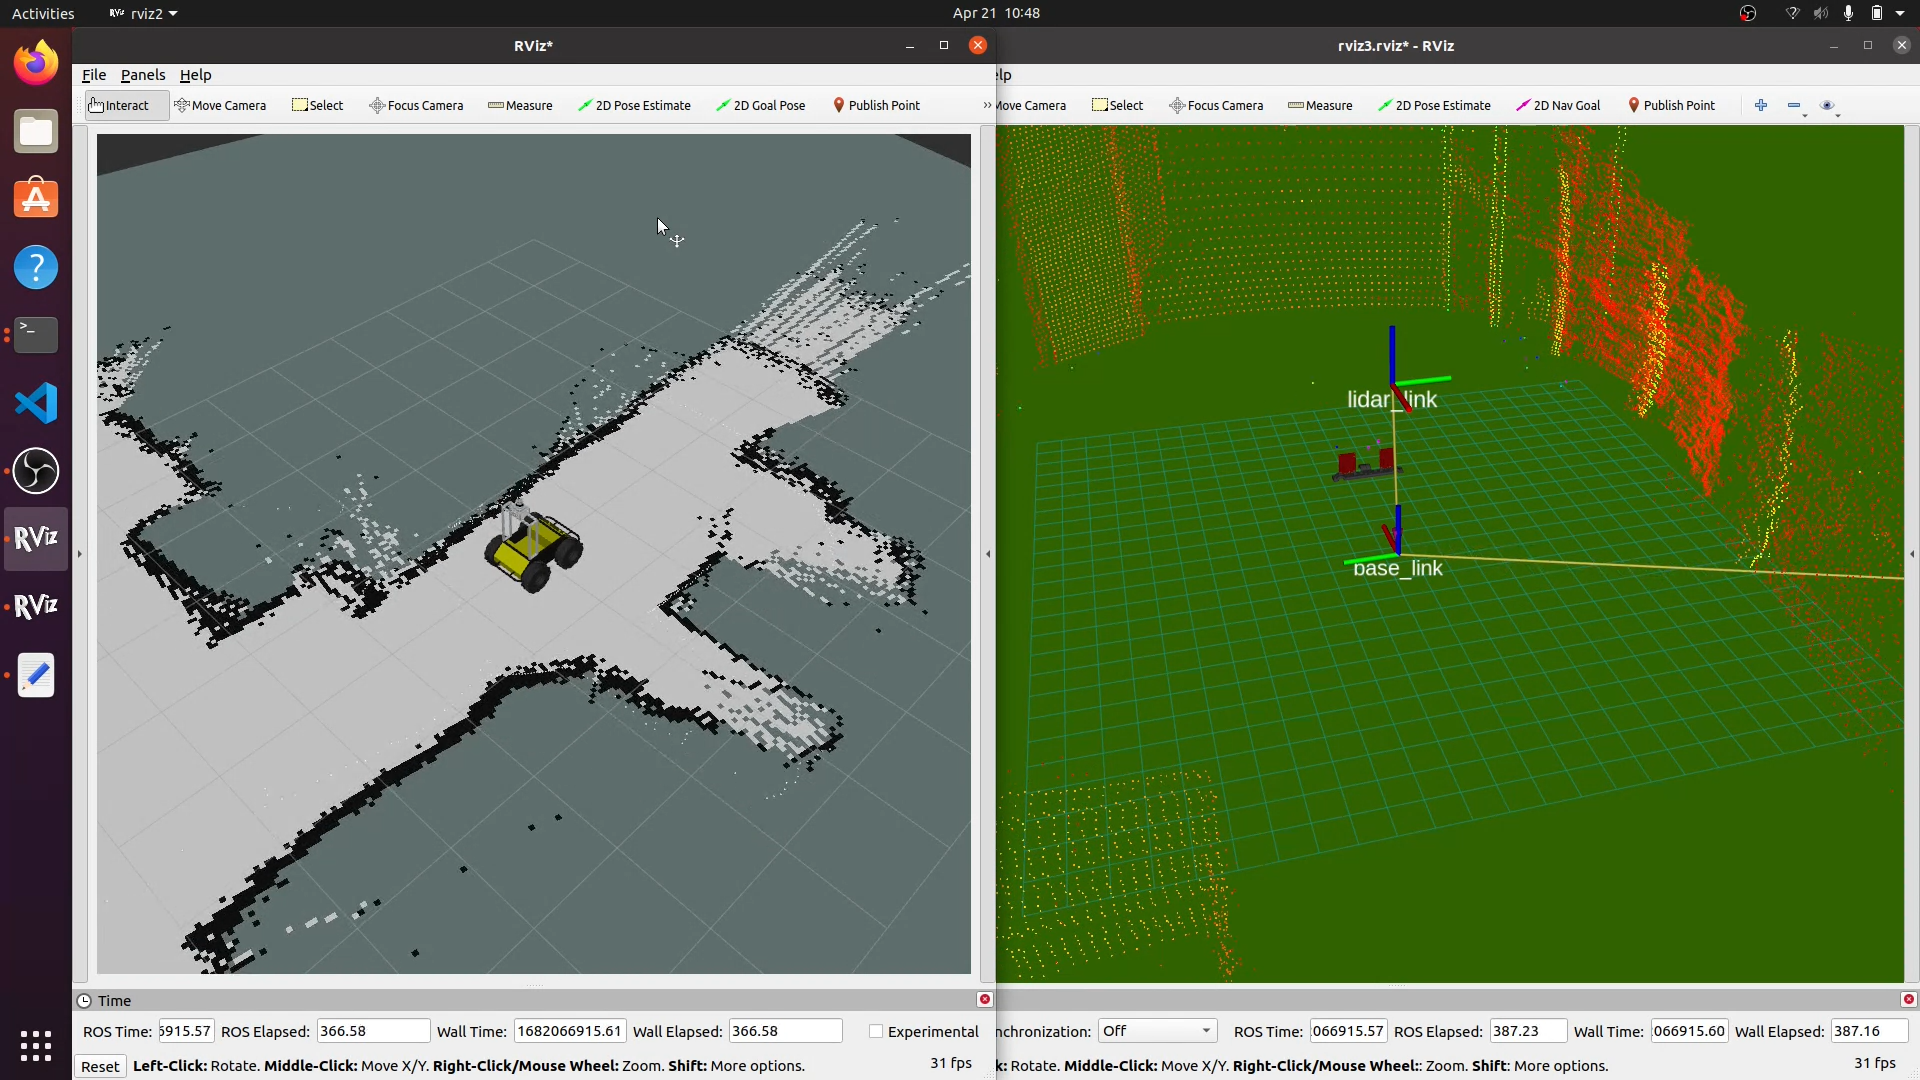
\includegraphics[width=\textwidth,trim={25cm 7cm 7cm 4cm},clip]{Figures/slamWithRadar.png}
        \caption{Zoomed in view of Rviz displaying the ranging data from the radars and the lidar. The bigger more colourful points are produced by the radars, the rest are from the lidar. The radar mount with two radar modules mounted are also visible. Based on figure \ref{fig:slamWithRadar}.}
        \label{fig:slamWithRadarRos1}
    \end{minipage}
\end{figure}

\begin{figure}[H]
    \centering
    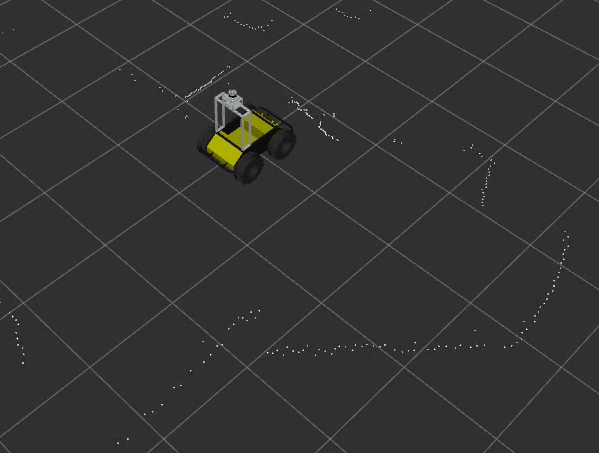
\includegraphics[width=0.8\textwidth]{Figures/radarAndLidarPointsInRos2.png}
    \caption{Better view of points representing the ranging data from ROS1, simmilar to the points in figure \ref{fig:slamWithRadarRos2}}
    \label{fig:radarAndLidarPointsInRos2}
\end{figure}

\section{Test with lidar (without radar)}
Figure \ref{fig:slamWithoutRadar} illustrate the SLAM-process of the test, but only based on range data from the lidar. The figure has similar properties to figure \ref{fig:slamWithRadarRos2} and \ref{fig:slamWithRadarRos1}, but the radar modules, and their data, is missing from Rviz (right side). The test uses a modified version of the algorithm, described in chapter \ref{sec:Algorithm}, where step 2.a, 2.c and 3 is not used, but the rest are.

\begin{figure}[H]
    \centering
    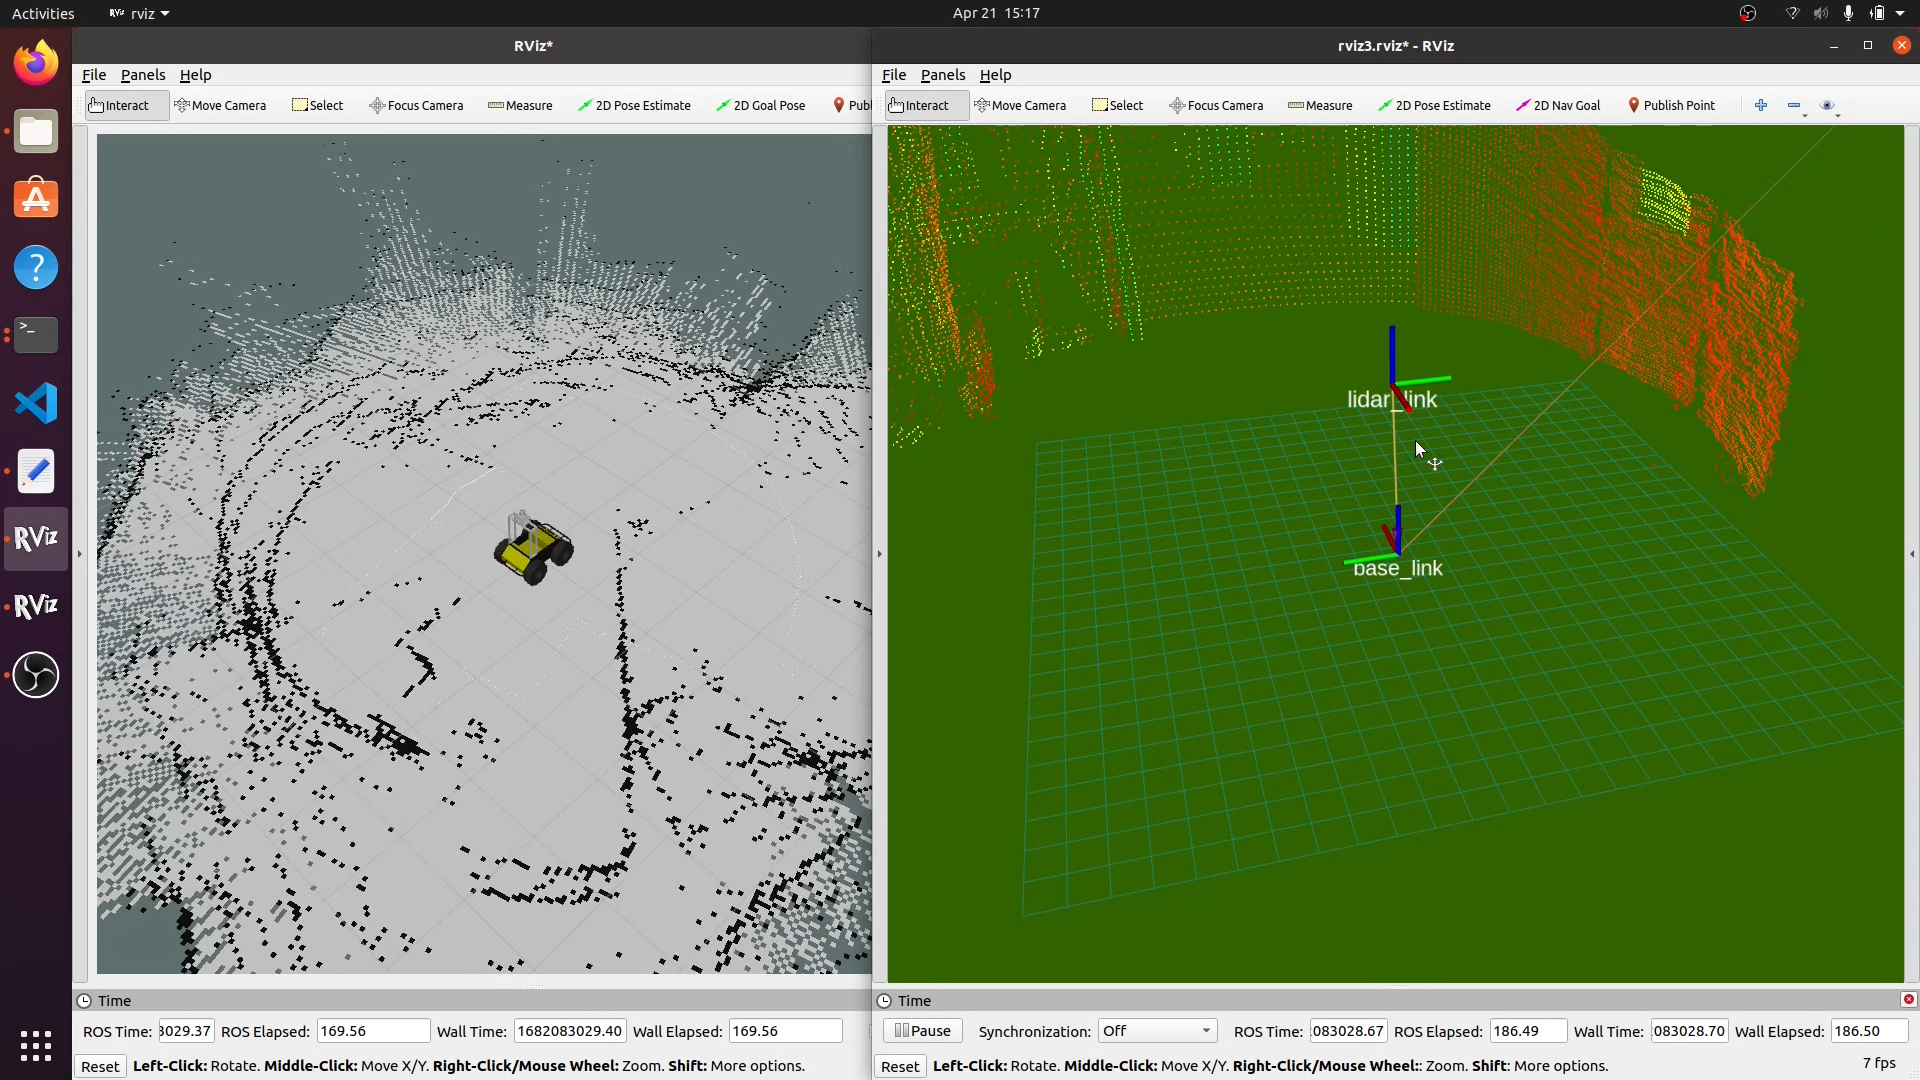
\includegraphics[width=\textwidth]{Figures/slamWithoutRadar.png}
    \caption{{View of ROS2 system (left) and ROS1 system (right) while SLAM runs without the radars. See figure \ref{fig:slamWithRadarRos1} and \ref{fig:slamWithRadarRos2} for a better understanding of figure.}}
    \label{fig:slamWithoutRadar}
\end{figure}

The testing position (displayed in figure \ref{fig:testSetup}) was assumed after a map was created. The test was den conducted as explained above. Figure \ref{fig:crashWithoutRadar} shows the aftermath of the test, where the Husky is standing on top of the backpack, after failing to detect and avoid it. Purple, pink and cyan areas displayed on the left side of the figure indicates detected objects, or areas to avoid. The colourful areas are part of the cost map.

\begin{figure}[H]
    \centering
    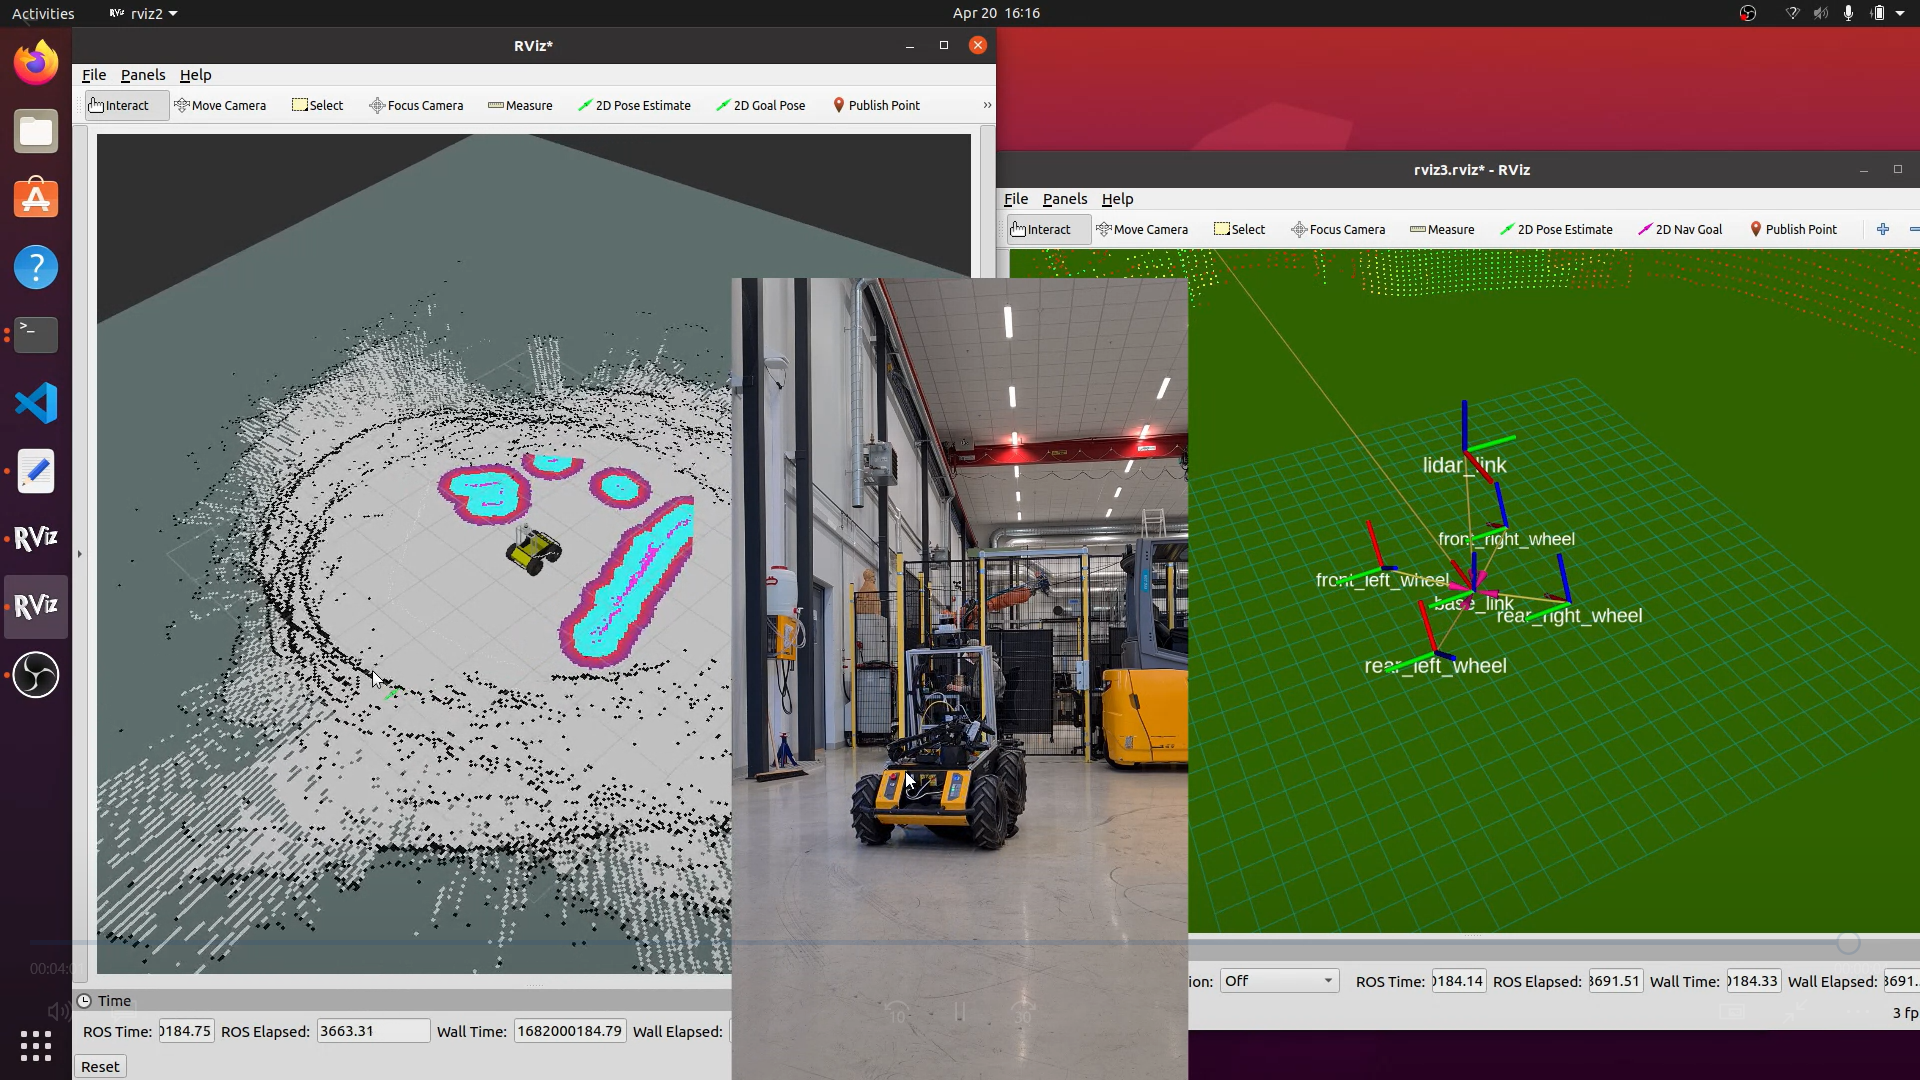
\includegraphics[width=\textwidth]{Figures/crashWithoutRadar.png}
    \caption{Failed collision avoidance test. The husky is standing on top of the backpack. Purple, pink and cyan areas indicating detected objects (cost map).}
    \label{fig:crashWithoutRadar}
\end{figure}

Figure \ref{fig:preCrashWithoutRadar} was captured just moments before \ref{fig:crashWithoutRadar}, where the backpack is not visible on the cost map. 

\begin{figure}[H]
    \centering
    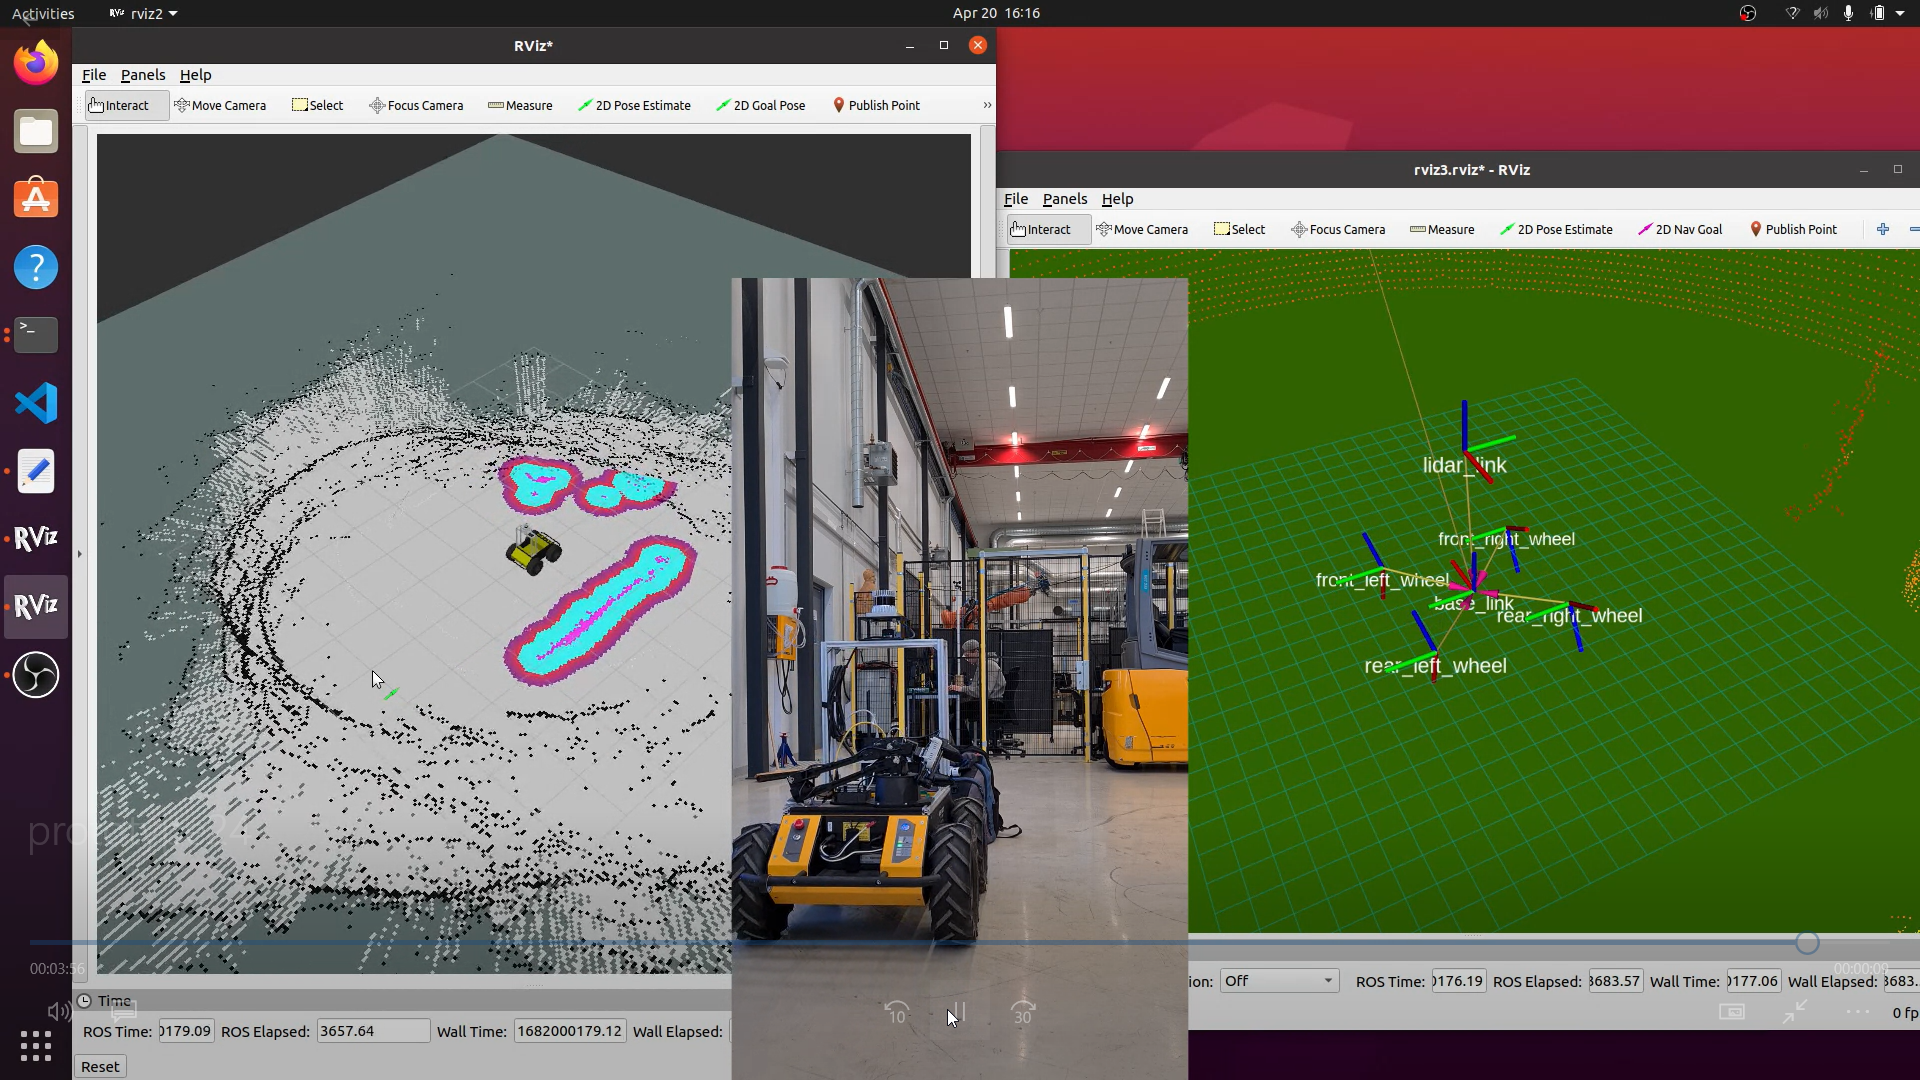
\includegraphics[width=\textwidth]{Figures/preCrashWithoutRadar.png}
    \caption{Failed collision avoidance test. Moments before failure. See figure \ref{fig:crashWithoutRadar} for collision.}
    \label{fig:preCrashWithoutRadar}
\end{figure}

\section{Test with radar and lidar}
Figure \ref{fig:slamWithRadar} displays the SLAM part of the test, but now with the radars. The test uses all of the steps of the algorithm described in chapter \ref{sec:Algorithm}.

\begin{figure}[H]
    \centering
    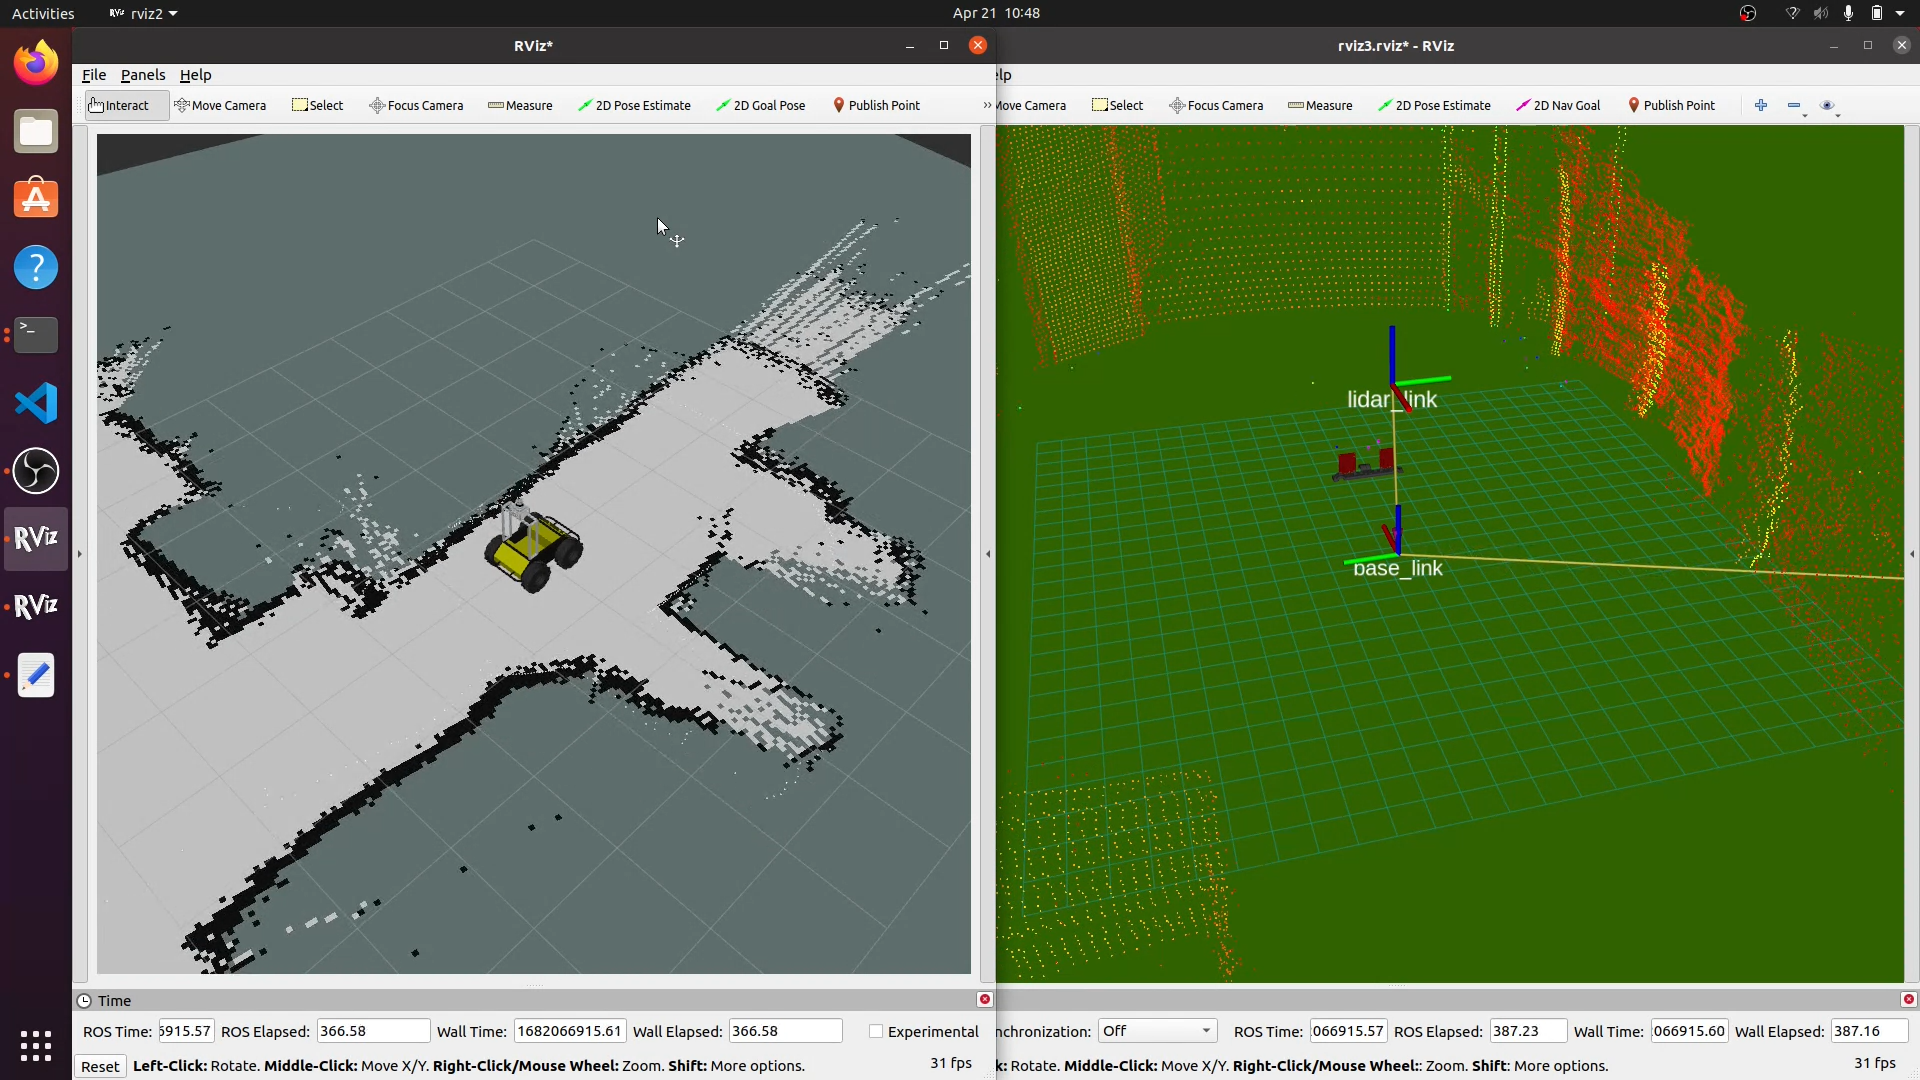
\includegraphics[width=\textwidth]{Figures/slamWithRadar.png}
    \caption{View of ROS2 system (left) and ROS1 system (right) while SLAM runs with the radars and the lidar. See figure \ref{fig:slamWithRadarRos1} and \ref{fig:slamWithRadarRos2} for more detail.}
    \label{fig:slamWithRadar}
\end{figure}

The test procedure was conducted similarly to above with the new map and radars activated. Figure \ref{fig:crashWithRadar} shows the aftermath of the test, where the Husky has stopped in front of the backpack. One can barley make out the colourful spheres that represents the radars' detection of the backpack.

\begin{figure}[H]
    \centering
    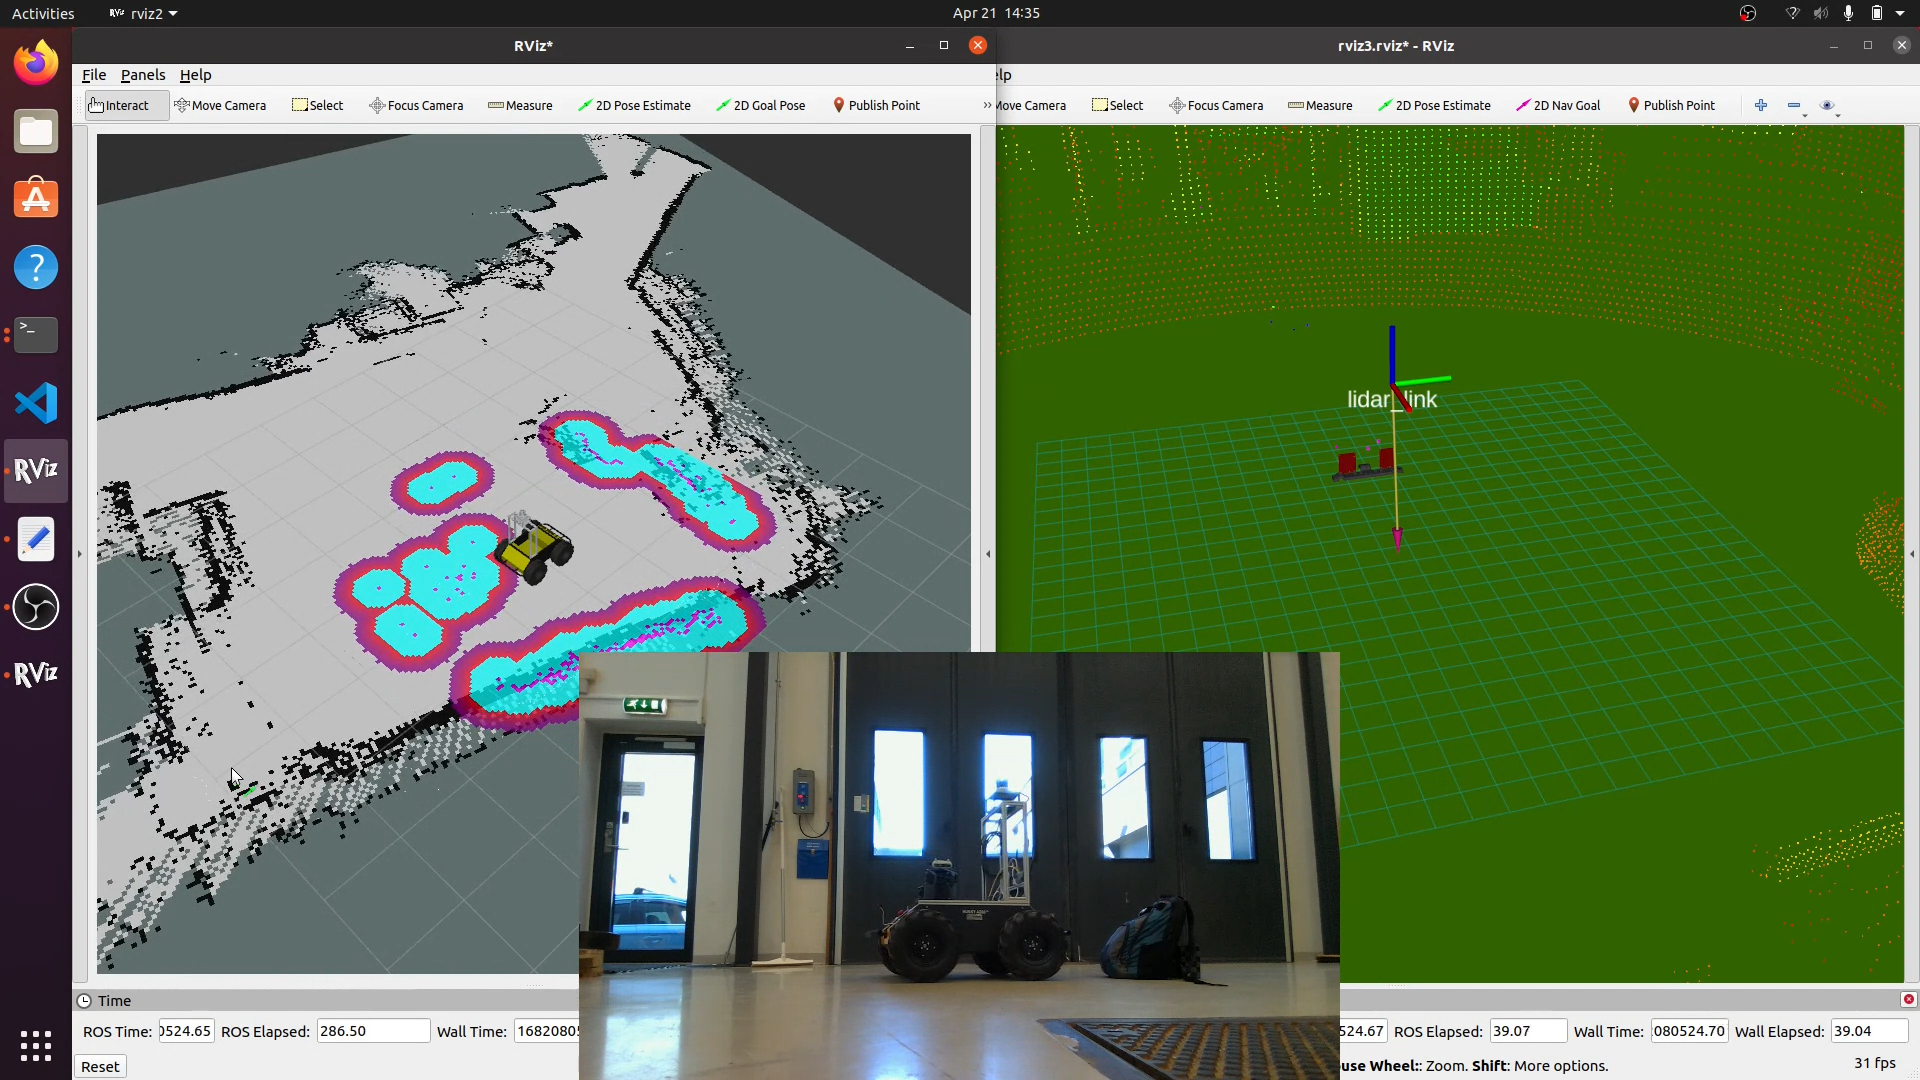
\includegraphics[width=\textwidth]{Figures/crashWithRadar.png}
    \caption{Husky standing still after stopping in front detected object, see figure \ref{fig:crashWithoutRadar}, \ref{fig:slamWithRadarRos2} and \ref{fig:slamWithRadarRos1} for better understanding}
    \label{fig:crashWithRadar}
\end{figure}



%\chapter{Discussions}
%\chapter{Conclusions}



\appendix

\chapter{Project in MAS513}
\label{Appdix:MAS513}
\includepdf[pages=-]{appendices/MAS513_Project__Husky_Group.pdf} 

\chapter{rqt node-graph of ros1 system}
\label{Appdix:rqtROS1NB}
\newpage
\begin{figure}[H]
%\centering
\includesvg[scale=0.2, angle=-90]{Figures/ros/ros1graph_noBridge.svg}
  \caption{rqt node-graph of ros1 system}
  \label{fig:Appdix:rqt:ros1_noBridge}
\end{figure}

\section{lidar.launch}
\label{Appdix:lidar.launch}
\inputminted{xml}{ros_system/launch/src/Refrencesignal.m}


\printbibliography[
heading=bibintoc,
title={Bibliography}
]


\end{document}

